%%%
%%%
%%%
%%%%%%%%%%%%%%%%%%%%%%%%%%%%%%%%%%%%%%%%%%%%%%%%%%%%%
%%% Abstract for Robotic-Assisted Medical Imaging 
%%% [LINK]: https://sites.google.com/view/rami-icra-2023-workshop/home
%%% Important dates 
%%% Abstract Submission Deadline: ~15th March 2023~, 24th March 2023
%%% Author Notification: 1st April 2023
%%% Workshop Date: 29th May 2023
%%%
%%%
%%% 
%%%%%%%%%%%%%%%%%%%%%%%%%%%%%%%%%%%%%%%%%%%%%%%%%%%%%
%%% Instructions for overleaf project
%%% Overleaf might be new to you, but it is quite easy to use. 
%%% 1. Go to the section where you want to write up or to edit in the PDF paper and double click that will point you to the text editor. 
%%% 2. Make edition as in word, and
%%% 3. Press Ctrl+s to save and compile your changes in the PDF document.
%%% 4. After Ctrl+s, all should be saved and ready for others to see, to review, etc.
%%% Ps. Using percentage symbol is considered as comment and it is not appearing in the PDF version of the paper.
%%% Don't worry about adding new references `\cite{}`, we can add them later.
%%% Thanks, Miguel
%%%
%%%
%%%%%%%%%%%%%%%%%%%%%%%%%%%%%%%%%%%%%%%%%%%%%%%%%%%%%
%%% Github repository:
%%% The resources to reproduce this work are available at 
%%% [LINK]: https://github.com/mxochicale/rami-icra2023
%%%
%%%
%%%


%%%%%%%%%%%%%%%%%%%%%%%%%%%%%%%%%%%%%%%%%%%%%%%%%%%%%%%%%%%%%%%%%%%%%%%%%%%%%%%%
%2345678901234567890123456789012345678901234567890123456789012345678901234567890
%        1         2         3         4         5         6         7         8

%\documentclass[letterpaper, 10 pt, conference]{ieeeconf}  % Comment this line out if you need a4paper

\documentclass[a4paper, 10pt, conference]{ieeeconf}      % Use this line for a4 paper

\IEEEoverridecommandlockouts             % This command is only needed if 
% you want to use the \thanks command

\overrideIEEEmargins                                      % Needed to meet printer requirements.

%In case you encounter the following error:
%Error 1010 The PDF file may be corrupt (unable to open PDF file) OR
%Error 1000 An error occurred while parsing a contents stream. Unable to analyze the PDF file.
%This is a known problem with pdfLaTeX conversion filter. The file cannot be opened with acrobat reader
%Please use one of the alternatives below to circumvent this error by uncommenting one or the other
%\pdfobjcompresslevel=0
%\pdfminorversion=4

% See the \addtolength command later in the file to balance the column lengths
% on the last page of the document

% The following packages can be found on http:\\www.ctan.org
%\usepackage{graphics} % for pdf, bitmapped graphics files
%\usepackage{epsfig} % for postscript graphics files
%\usepackage{mathptmx} % assumes new font selection scheme installed
%\usepackage{times} % assumes new font selection scheme installed
%\usepackage{amsmath} % assumes amsmath package installed
%\usepackage{amssymb}  % assumes amsmath package installed
\usepackage{graphicx}
\graphicspath{{../figures}} 
%\usepackage[hidelinks]{hyperref}
\usepackage{hyperref}
\hypersetup{
    colorlinks=false,
    pdfborder={0 0 0}
}

\title{\LARGE \bf
%Towards automatic ultrasound-guidance procedures. %Added: Thu 23 Feb 16:08:53 GMT 2023
%Learning ultrasound-guidance procedures. %Added: Thu 23 Feb 16:08:53 GMT 2023
%Towards AI-based ultrasound-guidance procedures %Mon 27 Feb 17:55:33 GMT 2023
%Learning and quantifying ultrasound-guidance procedures %Mon 27 Feb 17:57:32 GMT 2023
%Towards the Skill Transfer Learning of Ultrasound-guidance Procedures %Mon  6 Mar 00:23:54 GMT 2023
%Learning Skills of Ultrasound-guidance procedures  %Mon  6 Mar 00:41:51 GMT 2023
%Towards Skill Transfer Learning of Ultrasound-guidance Procedures %Mon  6 Mar 18:39:17 GMT 2023
%%
%Towards Reproducible Skill Transfer Learning 
%%Hardware and Software 
%Framework of Ultrasound-guidance Procedures %Mon  6 Mar 19:10:51 GMT 2023
%%
%Towards Reproducible Frameworks for Skill Transfer Learning of Ultrasound-guidance Procedures %Wed 15 Mar 17:41:03 GMT 2023
%Towards Reproducible Frameworks for Skill Transfer Learning of Robotic Ultrasound-guidance Procedures %Fri 17 Mar 17:15:29 GMT 2023
%Towards Simpler Frameworks for Skill Transfer Learning of \\ Robotic Ultrasound-guidance Procedures %Sat 18 Mar 23:43:33 GMT 2023
% Towards Simpler Frameworks of Skill Transfer Learning for \\ Robotic Ultrasound-guidance Procedures %Sun 19 Mar 00:14:16 GMT 2023
% Towards a Framework of Skill Transfer Learning for \\ Robotic Ultrasound-guidance Procedures %Sat 25 Mar 09:00:24 GMT 2023
Towards a Simple Framework of Skill Transfer Learning for \\ Robotic Ultrasound-guidance Procedures %Tue 28 Mar 23:11:49 BST 2023
}

\author{Tsz Yan Leung$^{1}$ and Miguel Xochicale$^{2}$% <-this % stops a space
% \author{[ADD CO-AUTHORS] and Miguel Xochicale$^{2}$% <-this % stops a space
%\thanks{*This work was not supported by any organization}% <-this % stops a space
\thanks{$^{1}$
	King's College London, UK
       {\tt\small tsz\_yan.leung@kcl.ac.uk}}%
\thanks{$^{2}$
	Currently University College London, UK. 
        Previously King's College London, UK.
        {\tt\small m.xochicale@ucl.ac.uk}}%
}


\begin{document}
\maketitle
\thispagestyle{empty}
\pagestyle{empty}


%%%%%%%%%%%%%%%%%%%%%%%%%%%%%%%%%%%%%%%%%%%%%%%%%%%%%%%%%%%%%%%%%%%%%%%%%%%%%%%%
\begin{abstract}
In this paper, we present a simple framework of skill transfer learning for robotic ultrasound-guidance procedures.
We briefly review challenges in skill transfer learning for robotic ultrasound-guidance procedures.
We then identify the need of appropriate sampling techniques, computationally efficient neural networks models that lead to the proposal of a simple framework of skill transfer learning for real-time applications in robotic ultrasound-guidance procedures.
We present pilot experiments from two participants (one experienced clinician and one non-clinician) looking for an optimal scanning plane of the four-chamber cardiac view from a fetal phantom.
We analysed ultrasound image frames, time series of texture image features and quaternions and found that the experienced clinician performed the procedure in a quicker and smoother way compared to lengthy and non-constant movements from non-clinicians.
For future work, we pointed out
the need of pruned and quantised neural network models
for real-time applications in robotic ultrasound-guidance
procedure.
The resources to reproduce this work are available at \url{https://github.com/mxochicale/rami-icra2023}.
\end{abstract}


%%%KEYWORDS 
% Image-guided intervention
% Robotic US imaging
% Autonomous medical imaging system

%%%%%%%%%%%%%%%%%%%%%%%%%%%%%%%%%%%%%%%%%%%%%%%%%%%%%%%%%%%%%%%%%%%%%%%%%%%%%%%%
\section{INTRODUCTION}
Ultrasound (US) imaging is a popular imaging modality because of its affordability, 
non-ionising imaging, and real-time capabilities.
Recently, the field of ultrasound-guidance procedures has been advanced with the development of robotic ultrasound systems that range from tele-operated, semi-autonomous and fully autonomous~\cite{deng2021, vonHaxthausen2021, Gerlach2022}. 
% Ipsen2021 leave out for future work
However, there are still scientific and technical challenges in robotic ultrasound-guidance procedures: 
(a) traditional imaging is user-dependent, skill-dependant and device-dependent \cite{chen1997},
(b) traditional hardware for human motion tracking is usually expensive or cumbersome~\cite{Dressler2021}, and 
(c) frameworks are designed for specific types of sensors, clinical US devices, robots and operating systems~\cite{niu2022}.
Learning ultrasound skills from sonographers that look for the optimal scanning plane (OSP) is still an open challenge in robotic ultrasound-guidance procedures~\cite{deng2021}.
It is hypothesised that robotic ultrasound-guided procedures would require to be simple, less expensive and less cumbersome for skill transfer learning.
Hence, in this paper, we are proposing a simple framework of skill transfer learning for robotic ultrasound-guidance procedures.
This paper is divided into robotic ultrasound-guidance procedures, framework for sonographer skill transfer learning, results and conclusions with future work.

% \section{SIMPLE FRAMEWORK OF SONOGRAPHER SKILL TRANSFER LEARNING FOR ROBOTIC ULTRASOUND-GUIDANCE PROCEDURES}
\section{ROBOTIC ULTRASOUND-GUIDANCE PROCEDURES}
Robotic ultrasound systems are actively investigated for teleoperatation, semi-autonomous and fully autonomous modalities~\cite{vonHaxthausen2021}.
For instance, Deng et al. proposed a multi-modal task learning architecture for ultrasound scanning skills with input data from ultrasound images, force and probe pose, stating the challenge of real-time guidance due to computational signal processing~\cite{deng2021}.
Robotic US-guidance radiation therapy for lesion in abdomen has been successful using CNN-based search.
However, treatment plans without US-robot guidance are still superior to robotic US-guidance because of the quality of acquired ultrasound images~\cite{Gerlach2022}.
% Recently, robotic minimally invasive surgery has been investigated with silica gel phantoms where the optical tracking system, from Vicon Motion Systems Ltd, was prone to deviations due to light occlusions~\cite{niu2022}.

%%---------------------------------(FIGURE)-------------------------------------
\begin{figure}[t]
\centering
\includegraphics[width=0.47\textwidth]{framework/outputs/drawing-v00} %%LOCAL/GITHUB
% 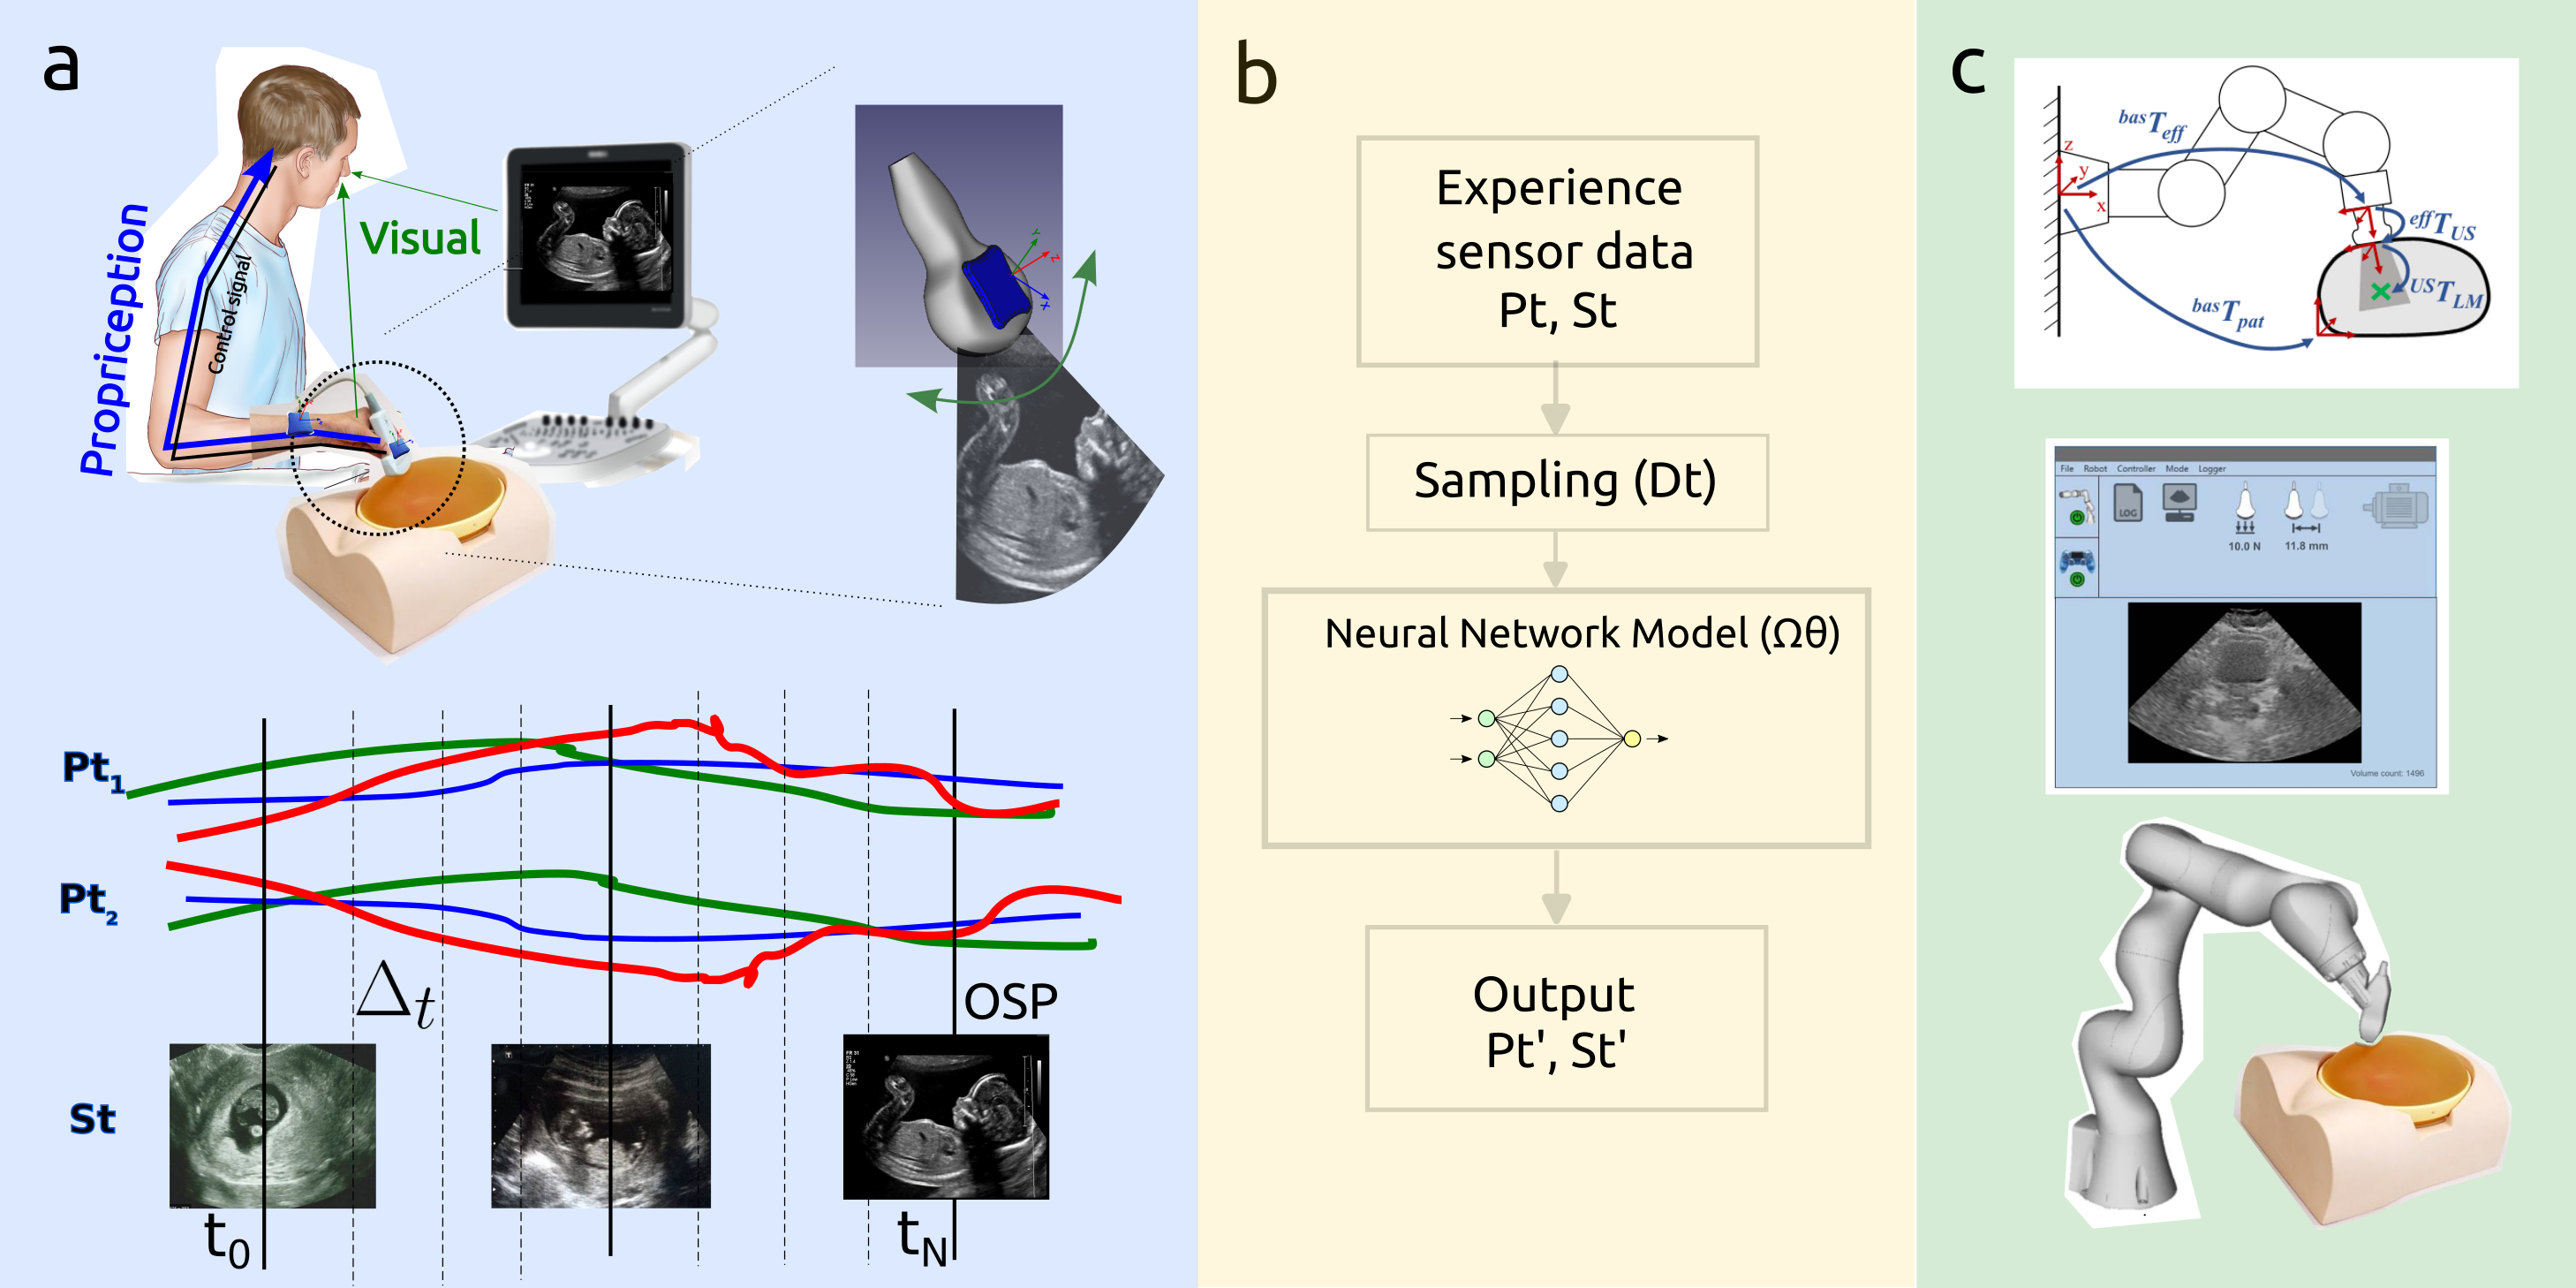
\includegraphics[width=0.47\textwidth]{fig-framework.png} %%OVERLEAF and ARXIV
    \caption{
            \textbf{(a)} Ultrasound-guidance procedures:
		sonographer operating an ultrasound machine with fetal phantom and sensor fusion signals from inertial sensors and ultrasound imaging;
            \textbf{(b)} Simple framework for skill transfer learning: 
		collecting experience with sensors ($Pt_n$ pose and $St$ Signal), sampling method for fusion sensor ($\Delta_t$), and identified the need of computational efficient neural network model ($\Omega_\theta$), and output for high-dimensional model ~\cite{deng2021}, and 
            %\textbf{(c)} 
            \textbf{(c)} Robotic ultrasound-guidance procedures:
		transformations, graphical user interface and simulation using robotic US-guidance light-weight 7 degrees-of-freedom robot (KUKA LBR Med 7)~\cite{Gerlach2022, Ipsen2021}.
       }
\label{fig:main}
\end{figure}
%%---------------------------------(FIGURE)------------------------------------

%%BLURS
%reproducible frameworks to address challenges on sustainability, reproducibly and good software/hardware practices.
%still be robustified by simplifying and making more effective procedures. 
%TOREVIEW~\cite{Ipsen2021}. 


\section{FRAMEWORK FOR SONOGRAPHER SKILL TRANSFER LEARNING}
%\subsection{Fusion-sensors}
Modelling the optimal scanning plane (OSP) requires ultrasound images, spacial locations and anatomical understanding from experienced sonographers (Fig~\ref{fig:main}a)~\cite{deng2021,vonHaxthausen2021}.
Current systems to model OPS are expensive and cumbersome leading to the need of smaller and low-cost systems~\cite{Dressler2021}. 
% This leads to systems that are expensive and 
% the need for simpler, affordable and less invasive framework for skill transfer learning. 
One potential avenue to reduce cost and ergonomic form factor is (a) the use of Inertial Measurement Units (IMU) to track probe position during US scanning procedures~\cite{PREVOST2018187}
and (b) the application of the appropriate fusion techniques of ultrasound video signal and motion signal from IMU for probe guidance~\cite{droste2020}, and (c) computationally efficient neural networks models~\cite{deng2021}.
Hence, we introduce a framework for sonographer skills transfer learning, considering: sampling technique and fusion sensor techniques (IMU and US) and discuss the need of real-time guidance with  pruned and quantised neural network models, feature extraction and transfer learning for robotic-ultrasound-guidance procedures (Fig~\ref{fig:main}b, c).
%%%BLURS

% Recently, Deng et al. investigated ultrasound skill learning with VGG-16 and fully connected layers by modelling relationships among US images, the probe pose and the contact force~\cite{deng2021}.
% However, real-time guidance is still a challenge due appropriate sampling techniques and the computational cost for large sensor samples.
% Hence, to address previous challenges in skill transfer learning, 

%Hence, considering the current trends towards the use of portable US scanners \cite{PREVOST2018187}.
%Droste et al. proposed a probe guidance system fusing 
%%was investigated to predict movement towards either the standard plane position or the next performed movements of a sonographer 

%%Similarly, having portable and non-obstrusive devices to track such image/orienation quality leads to essier clinical procedures [ADDREF].
%because of its small food print as well as the advantage oe being less expensive or add challenges in obstructions or magnetic disturbances.

%TOREVIEW 
%https://www.clinicalimaging.org/article/S0899-7071(21)00405-8/fulltext
%https://onlinelibrary.wiley.com/doi/abs/10.1002/jcu.23431?casa_token=Mq5YVW9UtLYAAAAA%3ARZ2sq111NUVdRyBDiTfWMdfWVtgoeTbAvw-DXPV5zwUD5IWzuu7VLAU2OgHEGobc0CO0b-S7Y2xQSaM
%https://aapm.onlinelibrary.wiley.com/doi/epdf/10.1002/mp.15432

\section{EXPERIMENTS: DESIGN AND RESULTS}
\subsection{Experiment setup}
Considering fetal biometry parameters from the NHS 20-week screening scan protocol and National Health Service (NHS) foetal anomaly screening programme (FASP)~\cite{NHS_england2022},
% NICE2022
we conducted a pilot experiment with two participants (one non-clinical and one clinical with 10 years of experience in echocardiography).
During the experiment, we asked participants to find the optimal scanning plane for the four chamber view of foetal ultrasound examination phantom ("SPACE FAN-ST", Kyoto Kagaku Co., Ltd, Kyoto, Japan).
We attached inertial sensors (LPMS-B2, LP-Research Inc., Tokyo, Japan) to a convex US probe to track the pose of the ultrasound image from a clinical ultrasound device (EPIQ 7G, Koninklijke Philips N.V., Amsterdam, Netherlands) with the use of a CPU laptop computer that streamed images via a USB framegrabber (Mirabox).

\subsection{Experimental results}
Fig~\ref{fig:results} shows the time series from one experienced clinician and one non-clinician while looking for an optimal scanning plane of the four-chamber view.
It can be noted that the expert took less time (1600 and 2500 samples) to find an optimal scanning plane whereas non-clinician took a greater time (5000 and 10000 samples).
Similarly, the time-series for the experienced clinician appear to be more smooth and consistent compared to the jerkiness of non-clinical participant. 
%%---------------------------------(FIGURE)-------------------------------------
\begin{figure}[t]
% \begin{figure*}[th] % two-column figure on desired page
\centering
\includegraphics[width=0.44\textwidth]{results-02-participants-02-trials/outputs/drawing-v00} %%LOCAL/GITHUB
% 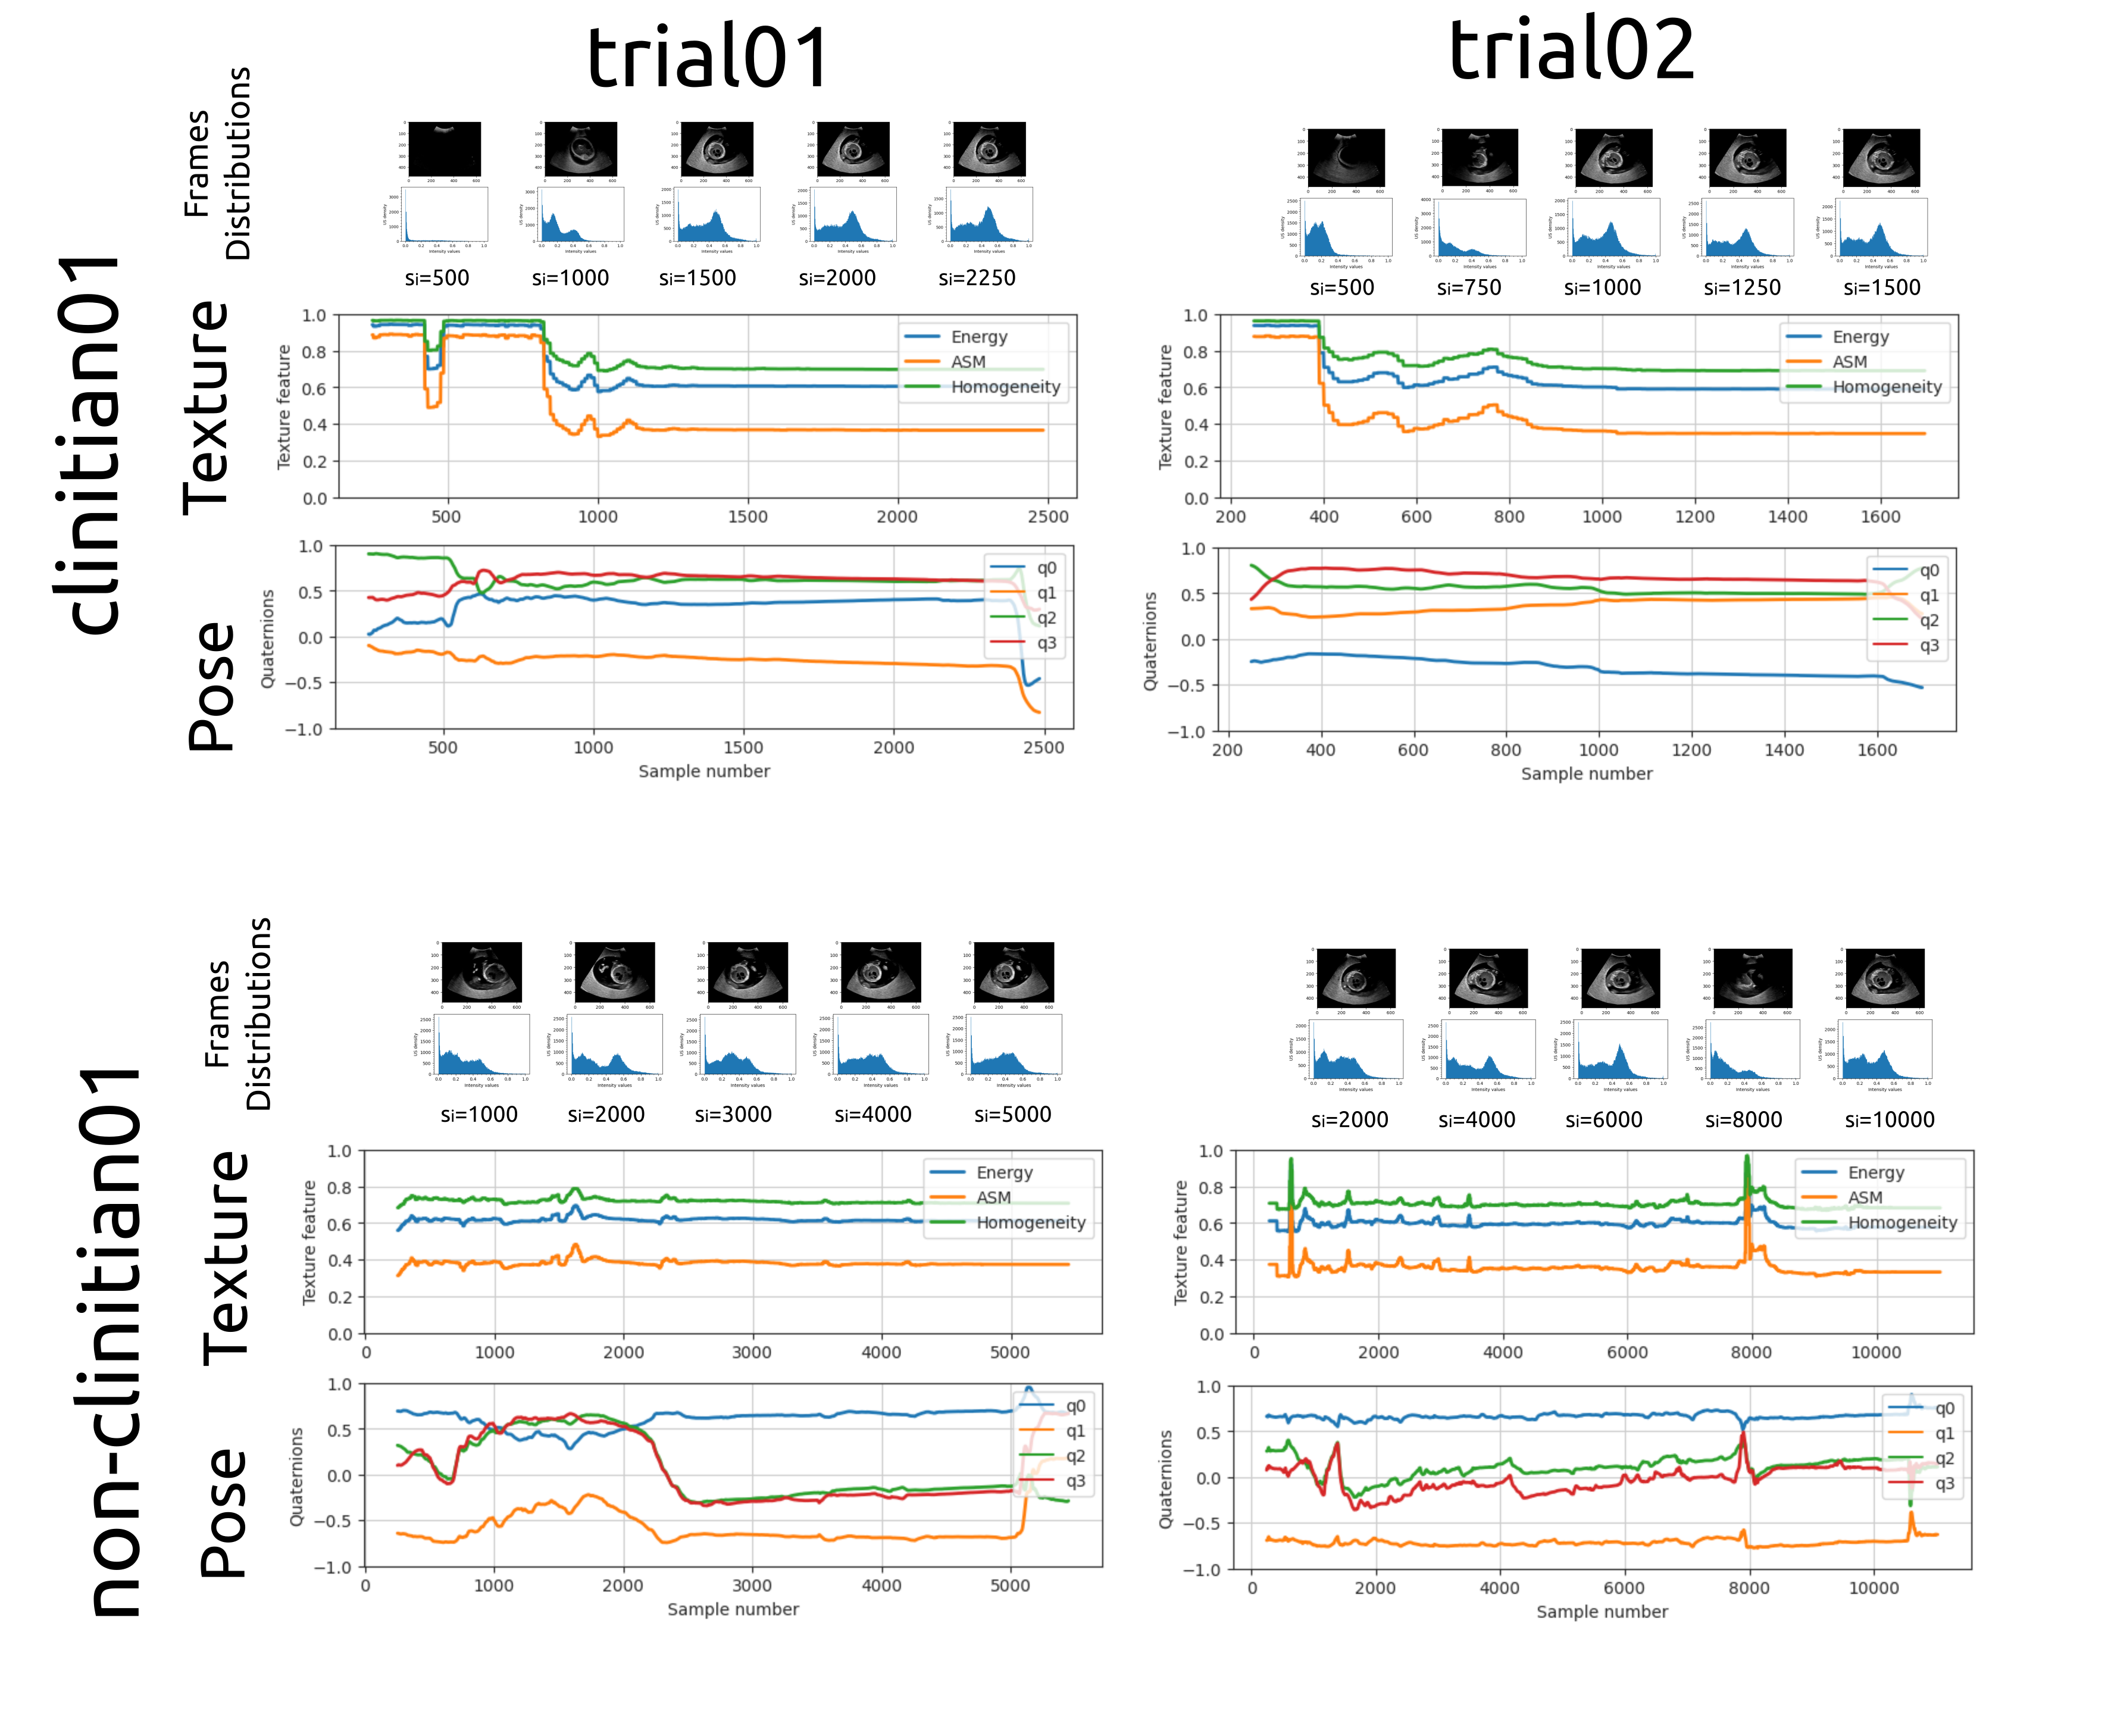
\includegraphics[width=0.44\textwidth]{fig-results-02-participants-02-trials.png} %%OVERLEAF and ARXIV
\caption{
Ultrasound image frames, image distributions, image texture features (energy, Angular Second Momentum ASM, and homogeneity) and pose time-series (quaternions) from one experienced clinician (clinician01) and one non-clinician (non-clinician01) in two trials (trial01 and trial02), looking for four-chamber optimal scanning plane. 
       } 
\label{fig:results}
% \end{figure*}
\end{figure}
%%---------------------------------(FIGURE)------------------------------------

%\subsection{Figures and Tables}
%Positioning Figures and Tables: Place figures and tables at the top and bottom of columns. Avoid placing them in the middle of columns. 
%Large figures and tables may span across both columns. 
%Figure captions should be below the figures; table heads should appear above the tables. 
%Insert figures and tables after they are cited in the text. 
%Use the abbreviation Fig. 1, even at the beginning of a sentence.
%\begin{table}[h]
%\caption{An Example of a Table}
%\label{table_example}
%\begin{center}
%\begin{tabular}{|c||c|}
%\hline
%One & Two\\
%\hline
%Three & Four\\
%\hline
%\end{tabular}
%\end{center}
%\end{table}
 
\section{CONCLUSIONS AND FUTURE WORK}
We have presented a simple framework of skill transfer learning for robotic ultrasound-guidance procedures.
We presented sensor fusion methods and sampling rate techniques for optimal scanning plane of the four-chamber view from two participants (one experienced clinician and one non-clinicians), where experienced clinician showed an smother and quicker procedure compare to a lengthy and non-constant movement of non-clinician.
For future work, we pointed out the need of pruned and quantised neural network models for real-time applications in robotic ultrasound-guidance procedure. 
% and a reproducible software/hardware pipeline to collect skills from clinicians to transfer them into a 
% simulated and r 

%%BLURS:FUTURE WORK 
%Hence, having appropriate methods to quantify such image and orientation quality in real-time leads with reliable clinical procedures is still an open challenge.
%NVIDIA Isaac Sim
%https://github.com/ArthurAllshire/HandTailor
%https://developer.nvidia.com/isaac-sim
%https://github.com/ankurhanda/dexpilot/tree/master

\addtolength{\textheight}{-12cm}   % This command serves to balance the column lengths
% on the last page of the document manually. It shortens
% the textheight of the last page by a suitable amount.
% This command does not take effect until the next page
% so it should come on the page before the last. Make
% sure that you do not shorten the textheight too much.

%%%%%%%%%%%%%%%%%%%%%%%%%%%%%%%%%%%%%%%%%%%%%%%%%%%%%%%%%%%%%%%%%%%%%%%%%%%%%%%%%
%\section*{APPENDIX}
%Appendixes should appear before the acknowledgment.

\section*{ACKNOWLEDGMENT}
Thanks to Tsz Yan Leung for her excellent research work  during her M.Sc. in Medical Physics and Engineering in 2022 at King's College London.
Thanks to Nhat Phung for volunteering as experienced sonographer in the experiments to identify optimal scanning plane of fetal four-chamber views at St Thomas' Hospital. 

%%%%%%%%%%%%%%%%%%%%%%%%%%%%%%%%%%%%%%%%%%%%%%%%%%%%%%%%%%%%%%%%%%%%%%%%%%%%%%%%
\bibliographystyle{IEEEtran}
\bibliography{../references/references}%%LOCAL/GITHUB
%\bibliography{references}%%OVERLEAF
% \bibliography{../../references/references}%%ARXIV
% %%%
%%%
%%%
%%%%%%%%%%%%%%%%%%%%%%%%%%%%%%%%%%%%%%%%%%%%%%%%%%%%%
%%% Abstract for Robotic-Assisted Medical Imaging 
%%% [LINK]: https://sites.google.com/view/rami-icra-2023-workshop/home
%%% Important dates 
%%% Abstract Submission Deadline: ~15th March 2023~, 24th March 2023
%%% Author Notification: 1st April 2023
%%% Workshop Date: 29th May 2023
%%%
%%%
%%% 
%%%%%%%%%%%%%%%%%%%%%%%%%%%%%%%%%%%%%%%%%%%%%%%%%%%%%
%%% Instructions for overleaf project
%%% Overleaf might be new to you, but it is quite easy to use. 
%%% 1. Go to the section where you want to write up or to edit in the PDF paper and double click that will point you to the text editor. 
%%% 2. Make edition as in word, and
%%% 3. Press Ctrl+s to save and compile your changes in the PDF document.
%%% 4. After Ctrl+s, all should be saved and ready for others to see, to review, etc.
%%% Ps. Using percentage symbol is considered as comment and it is not appearing in the PDF version of the paper.
%%% Don't worry about adding new references `\cite{}`, we can add them later.
%%% Thanks, Miguel
%%%
%%%
%%%%%%%%%%%%%%%%%%%%%%%%%%%%%%%%%%%%%%%%%%%%%%%%%%%%%
%%% Github repository:
%%% The resources to reproduce this work are available at 
%%% [LINK]: https://github.com/mxochicale/rami-icra2023
%%%
%%%
%%%


%%%%%%%%%%%%%%%%%%%%%%%%%%%%%%%%%%%%%%%%%%%%%%%%%%%%%%%%%%%%%%%%%%%%%%%%%%%%%%%%
%2345678901234567890123456789012345678901234567890123456789012345678901234567890
%        1         2         3         4         5         6         7         8

%\documentclass[letterpaper, 10 pt, conference]{ieeeconf}  % Comment this line out if you need a4paper

\documentclass[a4paper, 10pt, conference]{ieeeconf}      % Use this line for a4 paper

\IEEEoverridecommandlockouts             % This command is only needed if 
% you want to use the \thanks command

\overrideIEEEmargins                                      % Needed to meet printer requirements.

%In case you encounter the following error:
%Error 1010 The PDF file may be corrupt (unable to open PDF file) OR
%Error 1000 An error occurred while parsing a contents stream. Unable to analyze the PDF file.
%This is a known problem with pdfLaTeX conversion filter. The file cannot be opened with acrobat reader
%Please use one of the alternatives below to circumvent this error by uncommenting one or the other
%\pdfobjcompresslevel=0
%\pdfminorversion=4

% See the \addtolength command later in the file to balance the column lengths
% on the last page of the document

% The following packages can be found on http:\\www.ctan.org
%\usepackage{graphics} % for pdf, bitmapped graphics files
%\usepackage{epsfig} % for postscript graphics files
%\usepackage{mathptmx} % assumes new font selection scheme installed
%\usepackage{times} % assumes new font selection scheme installed
%\usepackage{amsmath} % assumes amsmath package installed
%\usepackage{amssymb}  % assumes amsmath package installed
\usepackage{graphicx}
\graphicspath{{../figures}} 
%\usepackage[hidelinks]{hyperref}
\usepackage{hyperref}
\hypersetup{
    colorlinks=false,
    pdfborder={0 0 0}
}

\title{\LARGE \bf
%Towards automatic ultrasound-guidance procedures. %Added: Thu 23 Feb 16:08:53 GMT 2023
%Learning ultrasound-guidance procedures. %Added: Thu 23 Feb 16:08:53 GMT 2023
%Towards AI-based ultrasound-guidance procedures %Mon 27 Feb 17:55:33 GMT 2023
%Learning and quantifying ultrasound-guidance procedures %Mon 27 Feb 17:57:32 GMT 2023
%Towards the Skill Transfer Learning of Ultrasound-guidance Procedures %Mon  6 Mar 00:23:54 GMT 2023
%Learning Skills of Ultrasound-guidance procedures  %Mon  6 Mar 00:41:51 GMT 2023
%Towards Skill Transfer Learning of Ultrasound-guidance Procedures %Mon  6 Mar 18:39:17 GMT 2023
%%
%Towards Reproducible Skill Transfer Learning 
%%Hardware and Software 
%Framework of Ultrasound-guidance Procedures %Mon  6 Mar 19:10:51 GMT 2023
%%
%Towards Reproducible Frameworks for Skill Transfer Learning of Ultrasound-guidance Procedures %Wed 15 Mar 17:41:03 GMT 2023
%Towards Reproducible Frameworks for Skill Transfer Learning of Robotic Ultrasound-guidance Procedures %Fri 17 Mar 17:15:29 GMT 2023
%Towards Simpler Frameworks for Skill Transfer Learning of \\ Robotic Ultrasound-guidance Procedures %Sat 18 Mar 23:43:33 GMT 2023
% Towards Simpler Frameworks of Skill Transfer Learning for \\ Robotic Ultrasound-guidance Procedures %Sun 19 Mar 00:14:16 GMT 2023
% Towards a Framework of Skill Transfer Learning for \\ Robotic Ultrasound-guidance Procedures %Sat 25 Mar 09:00:24 GMT 2023
Towards a Simple Framework of Skill Transfer Learning for \\ Robotic Ultrasound-guidance Procedures %Tue 28 Mar 23:11:49 BST 2023
}

\author{Tsz Yan Leung$^{1}$ and Miguel Xochicale$^{2}$% <-this % stops a space
% \author{[ADD CO-AUTHORS] and Miguel Xochicale$^{2}$% <-this % stops a space
%\thanks{*This work was not supported by any organization}% <-this % stops a space
\thanks{$^{1}$
	King's College London, UK
       {\tt\small tsz\_yan.leung@kcl.ac.uk}}%
\thanks{$^{2}$
	Currently University College London, UK. 
        Previously King's College London, UK.
        {\tt\small m.xochicale@ucl.ac.uk}}%
}


\begin{document}
\maketitle
\thispagestyle{empty}
\pagestyle{empty}


%%%%%%%%%%%%%%%%%%%%%%%%%%%%%%%%%%%%%%%%%%%%%%%%%%%%%%%%%%%%%%%%%%%%%%%%%%%%%%%%
\begin{abstract}
In this paper, we present a simple framework of skill transfer learning for robotic ultrasound-guidance procedures.
We briefly review challenges in skill transfer learning for robotic ultrasound-guidance procedures.
We then identify the need of appropriate sampling techniques, computationally efficient neural networks models that lead to the proposal of a simple framework of skill transfer learning for real-time applications in robotic ultrasound-guidance procedures.
We present pilot experiments from two participants (one experienced clinician and one non-clinician) looking for an optimal scanning plane of the four-chamber cardiac view from a fetal phantom.
We analysed ultrasound image frames, time series of texture image features and quaternions and found that the experienced clinician performed the procedure in a quicker and smoother way compared to lengthy and non-constant movements from non-clinicians.
For future work, we pointed out
the need of pruned and quantised neural network models
for real-time applications in robotic ultrasound-guidance
procedure.
The resources to reproduce this work are available at \url{https://github.com/mxochicale/rami-icra2023}.
\end{abstract}


%%%KEYWORDS 
% Image-guided intervention
% Robotic US imaging
% Autonomous medical imaging system

%%%%%%%%%%%%%%%%%%%%%%%%%%%%%%%%%%%%%%%%%%%%%%%%%%%%%%%%%%%%%%%%%%%%%%%%%%%%%%%%
\section{INTRODUCTION}
Ultrasound (US) imaging is a popular imaging modality because of its affordability, 
non-ionising imaging, and real-time capabilities.
Recently, the field of ultrasound-guidance procedures has been advanced with the development of robotic ultrasound systems that range from tele-operated, semi-autonomous and fully autonomous~\cite{deng2021, vonHaxthausen2021, Gerlach2022}. 
% Ipsen2021 leave out for future work
However, there are still scientific and technical challenges in robotic ultrasound-guidance procedures: 
(a) traditional imaging is user-dependent, skill-dependant and device-dependent \cite{chen1997},
(b) traditional hardware for human motion tracking is usually expensive or cumbersome~\cite{Dressler2021}, and 
(c) frameworks are designed for specific types of sensors, clinical US devices, robots and operating systems~\cite{niu2022}.
Learning ultrasound skills from sonographers that look for the optimal scanning plane (OSP) is still an open challenge in robotic ultrasound-guidance procedures~\cite{deng2021}.
It is hypothesised that robotic ultrasound-guided procedures would require to be simple, less expensive and less cumbersome for skill transfer learning.
Hence, in this paper, we are proposing a simple framework of skill transfer learning for robotic ultrasound-guidance procedures.
This paper is divided into robotic ultrasound-guidance procedures, framework for sonographer skill transfer learning, results and conclusions with future work.

% \section{SIMPLE FRAMEWORK OF SONOGRAPHER SKILL TRANSFER LEARNING FOR ROBOTIC ULTRASOUND-GUIDANCE PROCEDURES}
\section{ROBOTIC ULTRASOUND-GUIDANCE PROCEDURES}
Robotic ultrasound systems are actively investigated for teleoperatation, semi-autonomous and fully autonomous modalities~\cite{vonHaxthausen2021}.
For instance, Deng et al. proposed a multi-modal task learning architecture for ultrasound scanning skills with input data from ultrasound images, force and probe pose, stating the challenge of real-time guidance due to computational signal processing~\cite{deng2021}.
Robotic US-guidance radiation therapy for lesion in abdomen has been successful using CNN-based search.
However, treatment plans without US-robot guidance are still superior to robotic US-guidance because of the quality of acquired ultrasound images~\cite{Gerlach2022}.
% Recently, robotic minimally invasive surgery has been investigated with silica gel phantoms where the optical tracking system, from Vicon Motion Systems Ltd, was prone to deviations due to light occlusions~\cite{niu2022}.

%%---------------------------------(FIGURE)-------------------------------------
\begin{figure}[t]
\centering
% \includegraphics[width=0.47\textwidth]{framework/outputs/drawing-v00} %%LOCAL/GITHUB
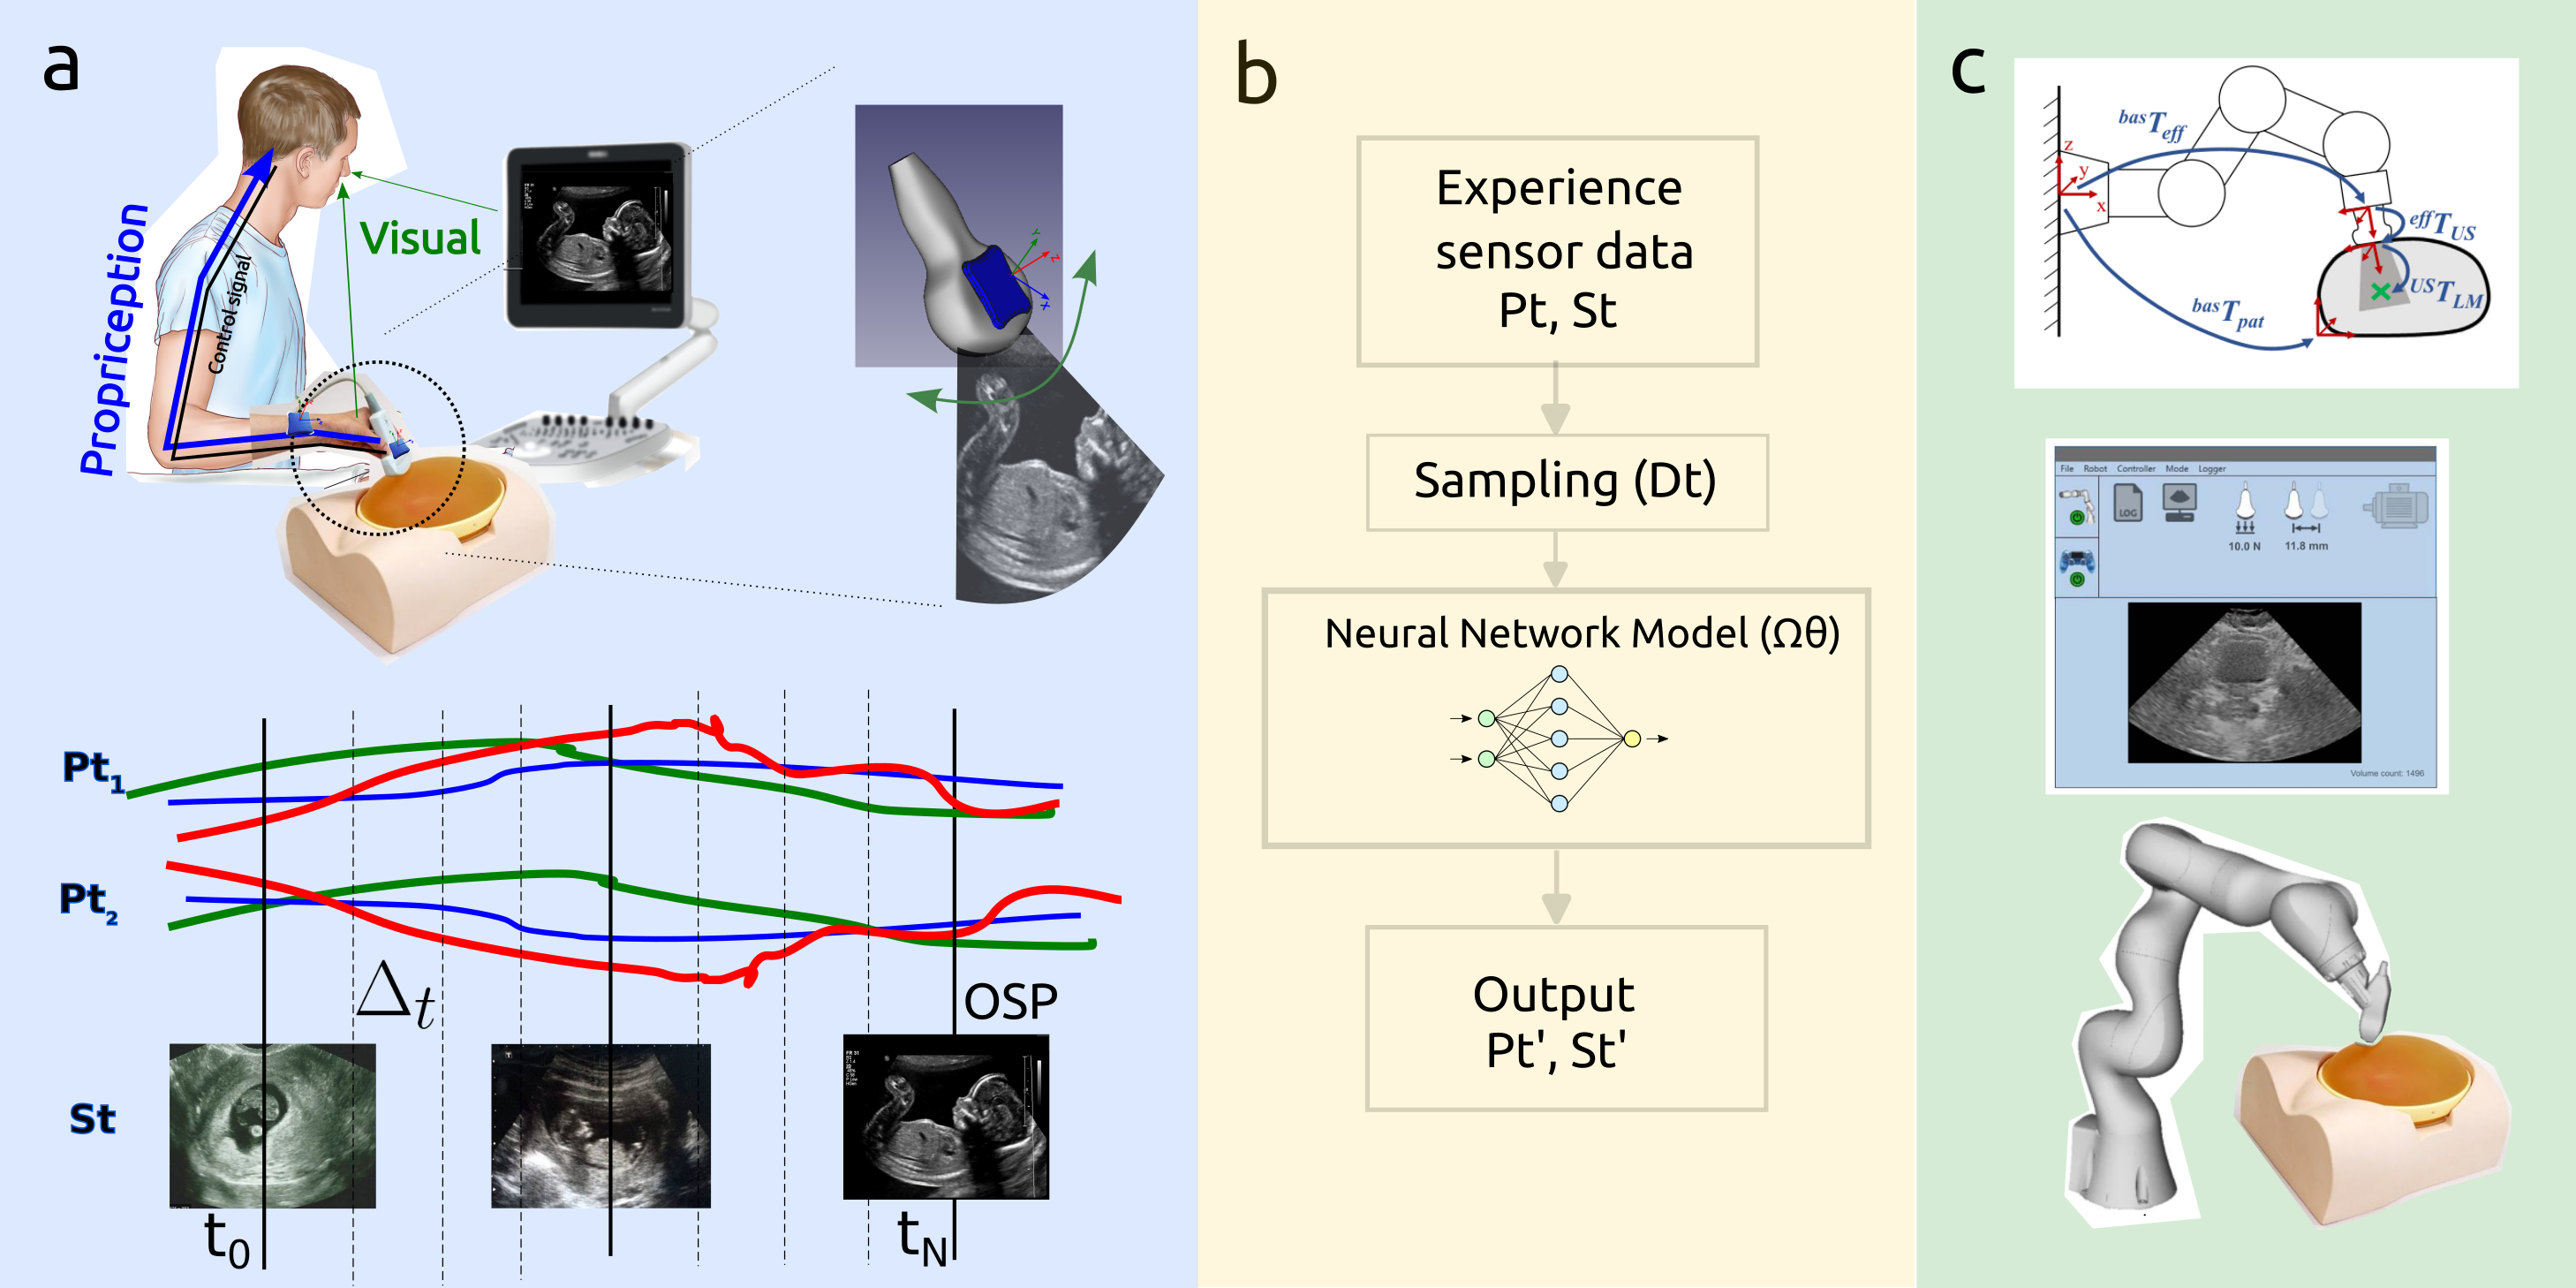
\includegraphics[width=0.47\textwidth]{fig-framework.png} %%OVERLEAF and ARXIV
    \caption{
            \textbf{(a)} Ultrasound-guidance procedures:
		sonographer operating an ultrasound machine with fetal phantom and sensor fusion signals from inertial sensors and ultrasound imaging;
            \textbf{(b)} Simple framework for skill transfer learning: 
		collecting experience with sensors ($Pt_n$ pose and $St$ Signal), sampling method for fusion sensor ($\Delta_t$), and identified the need of computational efficient neural network model ($\Omega_\theta$), and output for high-dimensional model ~\cite{deng2021}, and 
            %\textbf{(c)} 
            \textbf{(c)} Robotic ultrasound-guidance procedures:
		transformations, graphical user interface and simulation using robotic US-guidance light-weight 7 degrees-of-freedom robot (KUKA LBR Med 7)~\cite{Gerlach2022, Ipsen2021}.
       }
\label{fig:main}
\end{figure}
%%---------------------------------(FIGURE)------------------------------------

%%BLURS
%reproducible frameworks to address challenges on sustainability, reproducibly and good software/hardware practices.
%still be robustified by simplifying and making more effective procedures. 
%TOREVIEW~\cite{Ipsen2021}. 


\section{FRAMEWORK FOR SONOGRAPHER SKILL TRANSFER LEARNING}
%\subsection{Fusion-sensors}
Modelling the optimal scanning plane (OSP) requires ultrasound images, spacial locations and anatomical understanding from experienced sonographers (Fig~\ref{fig:main}a)~\cite{deng2021,vonHaxthausen2021}.
Current systems to model OPS are expensive and cumbersome leading to the need of smaller and low-cost systems~\cite{Dressler2021}. 
% This leads to systems that are expensive and 
% the need for simpler, affordable and less invasive framework for skill transfer learning. 
One potential avenue to reduce cost and ergonomic form factor is (a) the use of Inertial Measurement Units (IMU) to track probe position during US scanning procedures~\cite{PREVOST2018187}
and (b) the application of the appropriate fusion techniques of ultrasound video signal and motion signal from IMU for probe guidance~\cite{droste2020}, and (c) computationally efficient neural networks models~\cite{deng2021}.
Hence, we introduce a framework for sonographer skills transfer learning, considering: sampling technique and fusion sensor techniques (IMU and US) and discuss the need of real-time guidance with  pruned and quantised neural network models, feature extraction and transfer learning for robotic-ultrasound-guidance procedures (Fig~\ref{fig:main}b, c).
%%%BLURS

% Recently, Deng et al. investigated ultrasound skill learning with VGG-16 and fully connected layers by modelling relationships among US images, the probe pose and the contact force~\cite{deng2021}.
% However, real-time guidance is still a challenge due appropriate sampling techniques and the computational cost for large sensor samples.
% Hence, to address previous challenges in skill transfer learning, 

%Hence, considering the current trends towards the use of portable US scanners \cite{PREVOST2018187}.
%Droste et al. proposed a probe guidance system fusing 
%%was investigated to predict movement towards either the standard plane position or the next performed movements of a sonographer 

%%Similarly, having portable and non-obstrusive devices to track such image/orienation quality leads to essier clinical procedures [ADDREF].
%because of its small food print as well as the advantage oe being less expensive or add challenges in obstructions or magnetic disturbances.

%TOREVIEW 
%https://www.clinicalimaging.org/article/S0899-7071(21)00405-8/fulltext
%https://onlinelibrary.wiley.com/doi/abs/10.1002/jcu.23431?casa_token=Mq5YVW9UtLYAAAAA%3ARZ2sq111NUVdRyBDiTfWMdfWVtgoeTbAvw-DXPV5zwUD5IWzuu7VLAU2OgHEGobc0CO0b-S7Y2xQSaM
%https://aapm.onlinelibrary.wiley.com/doi/epdf/10.1002/mp.15432

\section{EXPERIMENTS: DESIGN AND RESULTS}
\subsection{Experiment setup}
Considering fetal biometry parameters from the NHS 20-week screening scan protocol and National Health Service (NHS) foetal anomaly screening programme (FASP)~\cite{NHS_england2022},
% NICE2022
we conducted a pilot experiment with two participants (one non-clinical and one clinical with 10 years of experience in echocardiography).
During the experiment, we asked participants to find the optimal scanning plane for the four chamber view of foetal ultrasound examination phantom ("SPACE FAN-ST", Kyoto Kagaku Co., Ltd, Kyoto, Japan).
We attached inertial sensors (LPMS-B2, LP-Research Inc., Tokyo, Japan) to a convex US probe to track the pose of the ultrasound image from a clinical ultrasound device (EPIQ 7G, Koninklijke Philips N.V., Amsterdam, Netherlands) with the use of a CPU laptop computer that streamed images via a USB framegrabber (Mirabox).

\subsection{Experimental results}
Fig~\ref{fig:results} shows the time series from one experienced clinician and one non-clinician while looking for an optimal scanning plane of the four-chamber view.
It can be noted that the expert took less time (1600 and 2500 samples) to find an optimal scanning plane whereas non-clinician took a greater time (5000 and 10000 samples).
Similarly, the time-series for the experienced clinician appear to be more smooth and consistent compared to the jerkiness of non-clinical participant. 
%%---------------------------------(FIGURE)-------------------------------------
\begin{figure}[t]
% \begin{figure*}[th] % two-column figure on desired page
\centering
% \includegraphics[width=0.44\textwidth]{results-02-participants-02-trials/outputs/drawing-v00} %%LOCAL/GITHUB
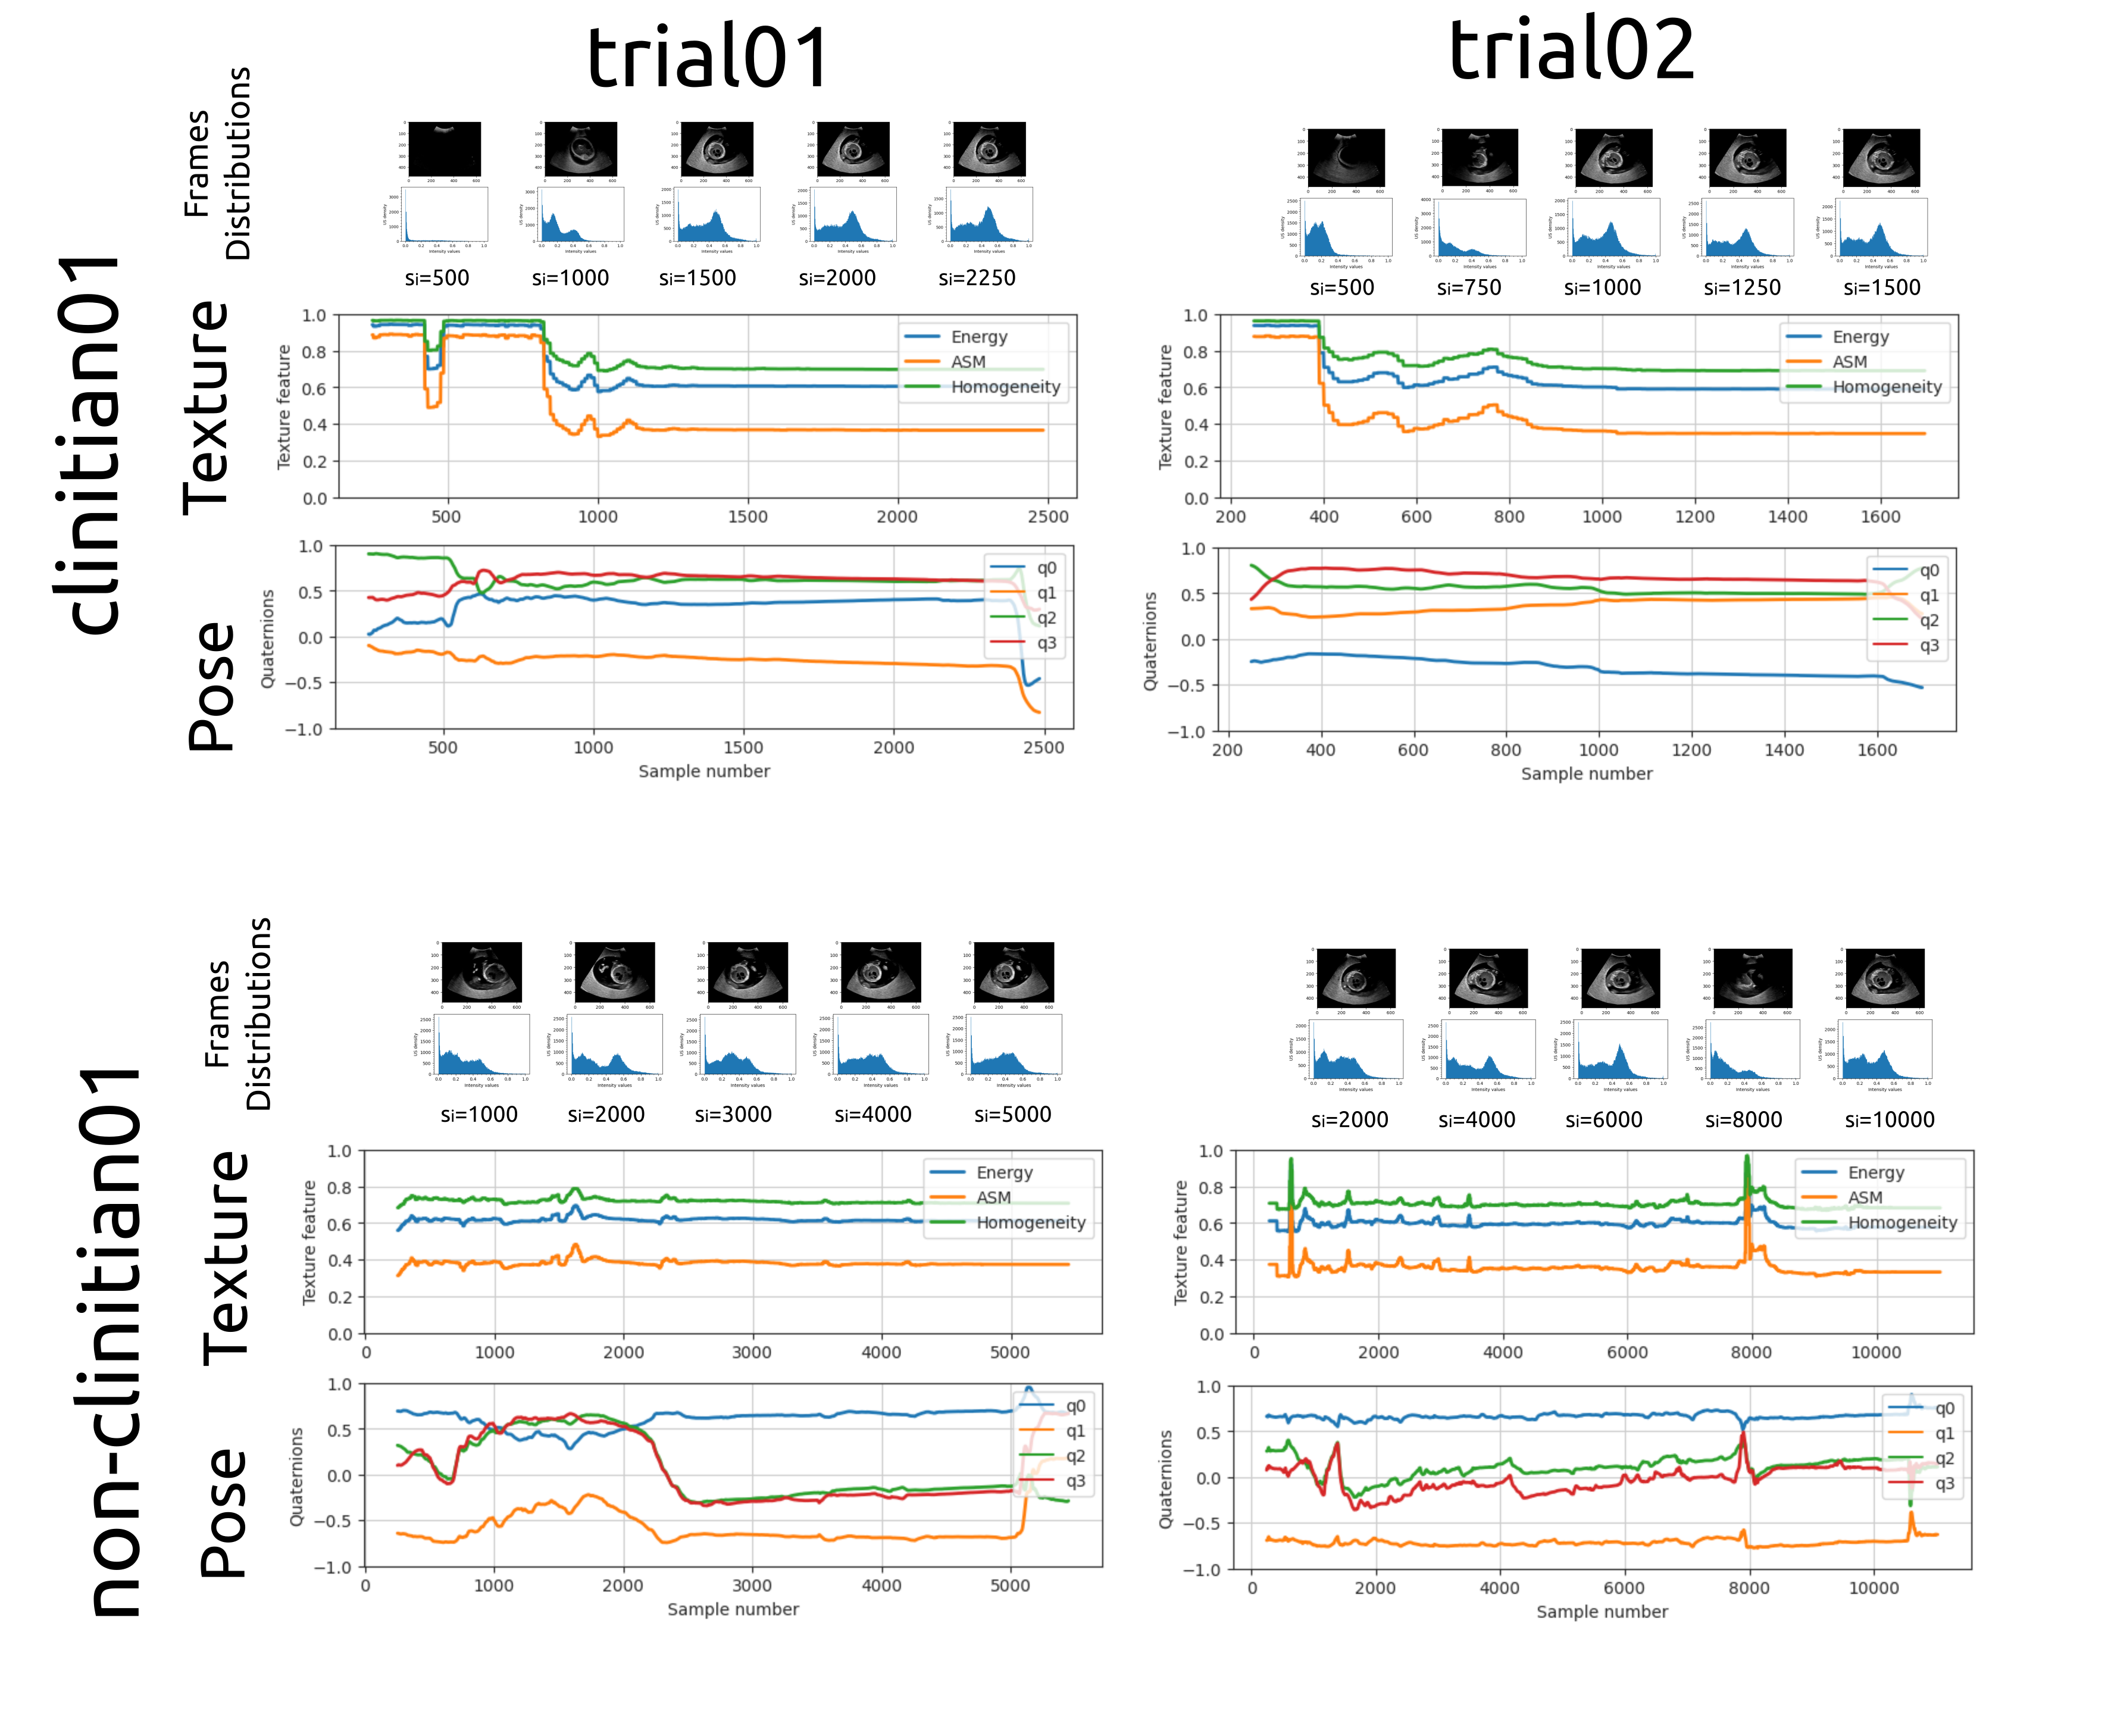
\includegraphics[width=0.44\textwidth]{fig-results-02-participants-02-trials.png} %%OVERLEAF and ARXIV
\caption{
Ultrasound image frames, image distributions, image texture features (energy, Angular Second Momentum ASM, and homogeneity) and pose time-series (quaternions) from one experienced clinician (clinician01) and one non-clinician (non-clinician01) in two trials (trial01 and trial02), looking for four-chamber optimal scanning plane. 
       } 
\label{fig:results}
% \end{figure*}
\end{figure}
%%---------------------------------(FIGURE)------------------------------------

%\subsection{Figures and Tables}
%Positioning Figures and Tables: Place figures and tables at the top and bottom of columns. Avoid placing them in the middle of columns. 
%Large figures and tables may span across both columns. 
%Figure captions should be below the figures; table heads should appear above the tables. 
%Insert figures and tables after they are cited in the text. 
%Use the abbreviation Fig. 1, even at the beginning of a sentence.
%\begin{table}[h]
%\caption{An Example of a Table}
%\label{table_example}
%\begin{center}
%\begin{tabular}{|c||c|}
%\hline
%One & Two\\
%\hline
%Three & Four\\
%\hline
%\end{tabular}
%\end{center}
%\end{table}
 
\section{CONCLUSIONS AND FUTURE WORK}
We have presented a simple framework of skill transfer learning for robotic ultrasound-guidance procedures.
We presented sensor fusion methods and sampling rate techniques for optimal scanning plane of the four-chamber view from two participants (one experienced clinician and one non-clinicians), where experienced clinician showed an smother and quicker procedure compare to a lengthy and non-constant movement of non-clinician.
For future work, we pointed out the need of pruned and quantised neural network models for real-time applications in robotic ultrasound-guidance procedure. 
% and a reproducible software/hardware pipeline to collect skills from clinicians to transfer them into a 
% simulated and r 

%%BLURS:FUTURE WORK 
%Hence, having appropriate methods to quantify such image and orientation quality in real-time leads with reliable clinical procedures is still an open challenge.
%NVIDIA Isaac Sim
%https://github.com/ArthurAllshire/HandTailor
%https://developer.nvidia.com/isaac-sim
%https://github.com/ankurhanda/dexpilot/tree/master

\addtolength{\textheight}{-12cm}   % This command serves to balance the column lengths
% on the last page of the document manually. It shortens
% the textheight of the last page by a suitable amount.
% This command does not take effect until the next page
% so it should come on the page before the last. Make
% sure that you do not shorten the textheight too much.

%%%%%%%%%%%%%%%%%%%%%%%%%%%%%%%%%%%%%%%%%%%%%%%%%%%%%%%%%%%%%%%%%%%%%%%%%%%%%%%%%
%\section*{APPENDIX}
%Appendixes should appear before the acknowledgment.

\section*{ACKNOWLEDGMENT}
Thanks to Tsz Yan Leung for her excellent research work  during her M.Sc. in Medical Physics and Engineering in 2022 at King's College London.
Thanks to Nhat Phung for volunteering as experienced sonographer in the experiments to identify optimal scanning plane of fetal four-chamber views at St Thomas' Hospital. 

%%%%%%%%%%%%%%%%%%%%%%%%%%%%%%%%%%%%%%%%%%%%%%%%%%%%%%%%%%%%%%%%%%%%%%%%%%%%%%%%
\bibliographystyle{IEEEtran}
% \bibliography{../references/references}%%LOCAL/GITHUB
%\bibliography{references}%%OVERLEAF
% \bibliography{../../references/references}%%ARXIV
%%%
%%%
%%%
%%%%%%%%%%%%%%%%%%%%%%%%%%%%%%%%%%%%%%%%%%%%%%%%%%%%%
%%% Abstract for Robotic-Assisted Medical Imaging 
%%% [LINK]: https://sites.google.com/view/rami-icra-2023-workshop/home
%%% Important dates 
%%% Abstract Submission Deadline: ~15th March 2023~, 24th March 2023
%%% Author Notification: 1st April 2023
%%% Workshop Date: 29th May 2023
%%%
%%%
%%% 
%%%%%%%%%%%%%%%%%%%%%%%%%%%%%%%%%%%%%%%%%%%%%%%%%%%%%
%%% Instructions for overleaf project
%%% Overleaf might be new to you, but it is quite easy to use. 
%%% 1. Go to the section where you want to write up or to edit in the PDF paper and double click that will point you to the text editor. 
%%% 2. Make edition as in word, and
%%% 3. Press Ctrl+s to save and compile your changes in the PDF document.
%%% 4. After Ctrl+s, all should be saved and ready for others to see, to review, etc.
%%% Ps. Using percentage symbol is considered as comment and it is not appearing in the PDF version of the paper.
%%% Don't worry about adding new references `\cite{}`, we can add them later.
%%% Thanks, Miguel
%%%
%%%
%%%%%%%%%%%%%%%%%%%%%%%%%%%%%%%%%%%%%%%%%%%%%%%%%%%%%
%%% Github repository:
%%% The resources to reproduce this work are available at 
%%% [LINK]: https://github.com/mxochicale/rami-icra2023
%%%
%%%
%%%


%%%%%%%%%%%%%%%%%%%%%%%%%%%%%%%%%%%%%%%%%%%%%%%%%%%%%%%%%%%%%%%%%%%%%%%%%%%%%%%%
%2345678901234567890123456789012345678901234567890123456789012345678901234567890
%        1         2         3         4         5         6         7         8

%\documentclass[letterpaper, 10 pt, conference]{ieeeconf}  % Comment this line out if you need a4paper

\documentclass[a4paper, 10pt, conference]{ieeeconf}      % Use this line for a4 paper

\IEEEoverridecommandlockouts             % This command is only needed if 
% you want to use the \thanks command

\overrideIEEEmargins                                      % Needed to meet printer requirements.

%In case you encounter the following error:
%Error 1010 The PDF file may be corrupt (unable to open PDF file) OR
%Error 1000 An error occurred while parsing a contents stream. Unable to analyze the PDF file.
%This is a known problem with pdfLaTeX conversion filter. The file cannot be opened with acrobat reader
%Please use one of the alternatives below to circumvent this error by uncommenting one or the other
%\pdfobjcompresslevel=0
%\pdfminorversion=4

% See the \addtolength command later in the file to balance the column lengths
% on the last page of the document

% The following packages can be found on http:\\www.ctan.org
%\usepackage{graphics} % for pdf, bitmapped graphics files
%\usepackage{epsfig} % for postscript graphics files
%\usepackage{mathptmx} % assumes new font selection scheme installed
%\usepackage{times} % assumes new font selection scheme installed
%\usepackage{amsmath} % assumes amsmath package installed
%\usepackage{amssymb}  % assumes amsmath package installed
\usepackage{graphicx}
\graphicspath{{../figures}} 
%\usepackage[hidelinks]{hyperref}
\usepackage{hyperref}
\hypersetup{
    colorlinks=false,
    pdfborder={0 0 0}
}

\title{\LARGE \bf
%Towards automatic ultrasound-guidance procedures. %Added: Thu 23 Feb 16:08:53 GMT 2023
%Learning ultrasound-guidance procedures. %Added: Thu 23 Feb 16:08:53 GMT 2023
%Towards AI-based ultrasound-guidance procedures %Mon 27 Feb 17:55:33 GMT 2023
%Learning and quantifying ultrasound-guidance procedures %Mon 27 Feb 17:57:32 GMT 2023
%Towards the Skill Transfer Learning of Ultrasound-guidance Procedures %Mon  6 Mar 00:23:54 GMT 2023
%Learning Skills of Ultrasound-guidance procedures  %Mon  6 Mar 00:41:51 GMT 2023
%Towards Skill Transfer Learning of Ultrasound-guidance Procedures %Mon  6 Mar 18:39:17 GMT 2023
%%
%Towards Reproducible Skill Transfer Learning 
%%Hardware and Software 
%Framework of Ultrasound-guidance Procedures %Mon  6 Mar 19:10:51 GMT 2023
%%
%Towards Reproducible Frameworks for Skill Transfer Learning of Ultrasound-guidance Procedures %Wed 15 Mar 17:41:03 GMT 2023
%Towards Reproducible Frameworks for Skill Transfer Learning of Robotic Ultrasound-guidance Procedures %Fri 17 Mar 17:15:29 GMT 2023
%Towards Simpler Frameworks for Skill Transfer Learning of \\ Robotic Ultrasound-guidance Procedures %Sat 18 Mar 23:43:33 GMT 2023
% Towards Simpler Frameworks of Skill Transfer Learning for \\ Robotic Ultrasound-guidance Procedures %Sun 19 Mar 00:14:16 GMT 2023
% Towards a Framework of Skill Transfer Learning for \\ Robotic Ultrasound-guidance Procedures %Sat 25 Mar 09:00:24 GMT 2023
Towards a Simple Framework of Skill Transfer Learning for \\ Robotic Ultrasound-guidance Procedures %Tue 28 Mar 23:11:49 BST 2023
}

\author{Tsz Yan Leung$^{1}$ and Miguel Xochicale$^{2}$% <-this % stops a space
% \author{[ADD CO-AUTHORS] and Miguel Xochicale$^{2}$% <-this % stops a space
%\thanks{*This work was not supported by any organization}% <-this % stops a space
\thanks{$^{1}$
	King's College London, UK
       {\tt\small tsz\_yan.leung@kcl.ac.uk}}%
\thanks{$^{2}$
	Currently University College London, UK. 
        Previously King's College London, UK.
        {\tt\small m.xochicale@ucl.ac.uk}}%
}


\begin{document}
\maketitle
\thispagestyle{empty}
\pagestyle{empty}


%%%%%%%%%%%%%%%%%%%%%%%%%%%%%%%%%%%%%%%%%%%%%%%%%%%%%%%%%%%%%%%%%%%%%%%%%%%%%%%%
\begin{abstract}
In this paper, we present a simple framework of skill transfer learning for robotic ultrasound-guidance procedures.
We briefly review challenges in skill transfer learning for robotic ultrasound-guidance procedures.
We then identify the need of appropriate sampling techniques, computationally efficient neural networks models that lead to the proposal of a simple framework of skill transfer learning for real-time applications in robotic ultrasound-guidance procedures.
We present pilot experiments from two participants (one experienced clinician and one non-clinician) looking for an optimal scanning plane of the four-chamber cardiac view from a fetal phantom.
We analysed ultrasound image frames, time series of texture image features and quaternions and found that the experienced clinician performed the procedure in a quicker and smoother way compared to lengthy and non-constant movements from non-clinicians.
For future work, we pointed out
the need of pruned and quantised neural network models
for real-time applications in robotic ultrasound-guidance
procedure.
The resources to reproduce this work are available at \url{https://github.com/mxochicale/rami-icra2023}.
\end{abstract}


%%%KEYWORDS 
% Image-guided intervention
% Robotic US imaging
% Autonomous medical imaging system

%%%%%%%%%%%%%%%%%%%%%%%%%%%%%%%%%%%%%%%%%%%%%%%%%%%%%%%%%%%%%%%%%%%%%%%%%%%%%%%%
\section{INTRODUCTION}
Ultrasound (US) imaging is a popular imaging modality because of its affordability, 
non-ionising imaging, and real-time capabilities.
Recently, the field of ultrasound-guidance procedures has been advanced with the development of robotic ultrasound systems that range from tele-operated, semi-autonomous and fully autonomous~\cite{deng2021, vonHaxthausen2021, Gerlach2022}. 
% Ipsen2021 leave out for future work
However, there are still scientific and technical challenges in robotic ultrasound-guidance procedures: 
(a) traditional imaging is user-dependent, skill-dependant and device-dependent \cite{chen1997},
(b) traditional hardware for human motion tracking is usually expensive or cumbersome~\cite{Dressler2021}, and 
(c) frameworks are designed for specific types of sensors, clinical US devices, robots and operating systems~\cite{niu2022}.
Learning ultrasound skills from sonographers that look for the optimal scanning plane (OSP) is still an open challenge in robotic ultrasound-guidance procedures~\cite{deng2021}.
It is hypothesised that robotic ultrasound-guided procedures would require to be simple, less expensive and less cumbersome for skill transfer learning.
Hence, in this paper, we are proposing a simple framework of skill transfer learning for robotic ultrasound-guidance procedures.
This paper is divided into robotic ultrasound-guidance procedures, framework for sonographer skill transfer learning, results and conclusions with future work.

% \section{SIMPLE FRAMEWORK OF SONOGRAPHER SKILL TRANSFER LEARNING FOR ROBOTIC ULTRASOUND-GUIDANCE PROCEDURES}
\section{ROBOTIC ULTRASOUND-GUIDANCE PROCEDURES}
Robotic ultrasound systems are actively investigated for teleoperatation, semi-autonomous and fully autonomous modalities~\cite{vonHaxthausen2021}.
For instance, Deng et al. proposed a multi-modal task learning architecture for ultrasound scanning skills with input data from ultrasound images, force and probe pose, stating the challenge of real-time guidance due to computational signal processing~\cite{deng2021}.
Robotic US-guidance radiation therapy for lesion in abdomen has been successful using CNN-based search.
However, treatment plans without US-robot guidance are still superior to robotic US-guidance because of the quality of acquired ultrasound images~\cite{Gerlach2022}.
% Recently, robotic minimally invasive surgery has been investigated with silica gel phantoms where the optical tracking system, from Vicon Motion Systems Ltd, was prone to deviations due to light occlusions~\cite{niu2022}.

%%---------------------------------(FIGURE)-------------------------------------
\begin{figure}[t]
\centering
% \includegraphics[width=0.47\textwidth]{framework/outputs/drawing-v00} %%LOCAL/GITHUB
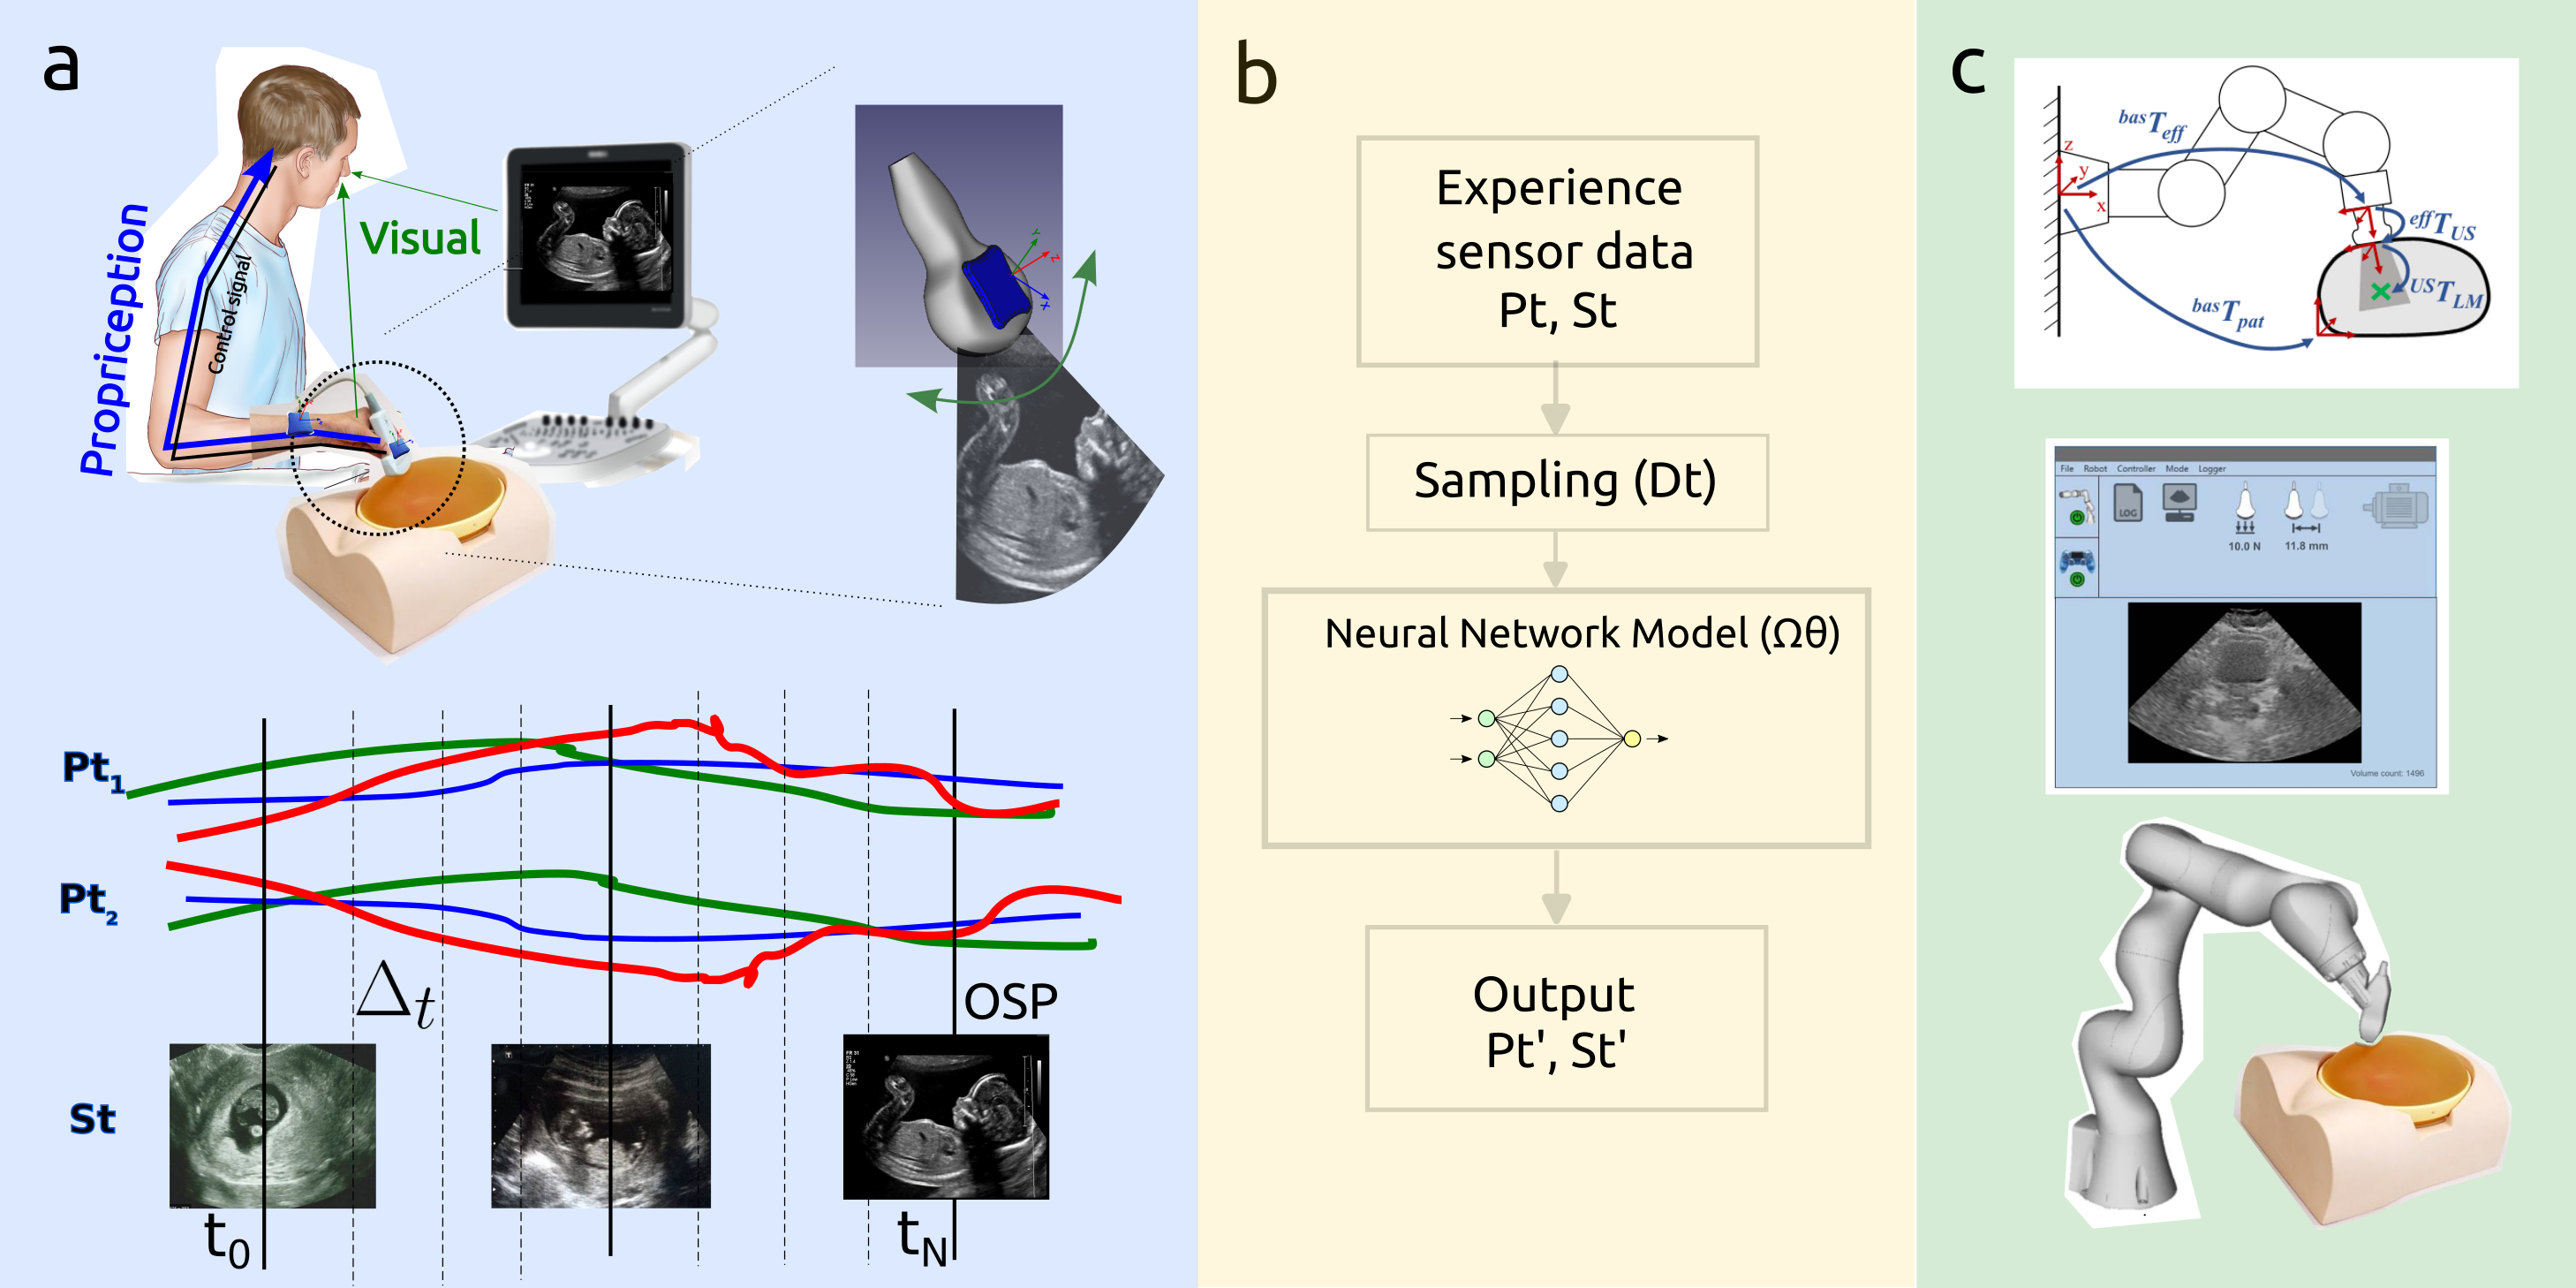
\includegraphics[width=0.47\textwidth]{fig-framework.png} %%OVERLEAF and ARXIV
    \caption{
            \textbf{(a)} Ultrasound-guidance procedures:
		sonographer operating an ultrasound machine with fetal phantom and sensor fusion signals from inertial sensors and ultrasound imaging;
            \textbf{(b)} Simple framework for skill transfer learning: 
		collecting experience with sensors ($Pt_n$ pose and $St$ Signal), sampling method for fusion sensor ($\Delta_t$), and identified the need of computational efficient neural network model ($\Omega_\theta$), and output for high-dimensional model ~\cite{deng2021}, and 
            %\textbf{(c)} 
            \textbf{(c)} Robotic ultrasound-guidance procedures:
		transformations, graphical user interface and simulation using robotic US-guidance light-weight 7 degrees-of-freedom robot (KUKA LBR Med 7)~\cite{Gerlach2022, Ipsen2021}.
       }
\label{fig:main}
\end{figure}
%%---------------------------------(FIGURE)------------------------------------

%%BLURS
%reproducible frameworks to address challenges on sustainability, reproducibly and good software/hardware practices.
%still be robustified by simplifying and making more effective procedures. 
%TOREVIEW~\cite{Ipsen2021}. 


\section{FRAMEWORK FOR SONOGRAPHER SKILL TRANSFER LEARNING}
%\subsection{Fusion-sensors}
Modelling the optimal scanning plane (OSP) requires ultrasound images, spacial locations and anatomical understanding from experienced sonographers (Fig~\ref{fig:main}a)~\cite{deng2021,vonHaxthausen2021}.
Current systems to model OPS are expensive and cumbersome leading to the need of smaller and low-cost systems~\cite{Dressler2021}. 
% This leads to systems that are expensive and 
% the need for simpler, affordable and less invasive framework for skill transfer learning. 
One potential avenue to reduce cost and ergonomic form factor is (a) the use of Inertial Measurement Units (IMU) to track probe position during US scanning procedures~\cite{PREVOST2018187}
and (b) the application of the appropriate fusion techniques of ultrasound video signal and motion signal from IMU for probe guidance~\cite{droste2020}, and (c) computationally efficient neural networks models~\cite{deng2021}.
Hence, we introduce a framework for sonographer skills transfer learning, considering: sampling technique and fusion sensor techniques (IMU and US) and discuss the need of real-time guidance with  pruned and quantised neural network models, feature extraction and transfer learning for robotic-ultrasound-guidance procedures (Fig~\ref{fig:main}b, c).
%%%BLURS

% Recently, Deng et al. investigated ultrasound skill learning with VGG-16 and fully connected layers by modelling relationships among US images, the probe pose and the contact force~\cite{deng2021}.
% However, real-time guidance is still a challenge due appropriate sampling techniques and the computational cost for large sensor samples.
% Hence, to address previous challenges in skill transfer learning, 

%Hence, considering the current trends towards the use of portable US scanners \cite{PREVOST2018187}.
%Droste et al. proposed a probe guidance system fusing 
%%was investigated to predict movement towards either the standard plane position or the next performed movements of a sonographer 

%%Similarly, having portable and non-obstrusive devices to track such image/orienation quality leads to essier clinical procedures [ADDREF].
%because of its small food print as well as the advantage oe being less expensive or add challenges in obstructions or magnetic disturbances.

%TOREVIEW 
%https://www.clinicalimaging.org/article/S0899-7071(21)00405-8/fulltext
%https://onlinelibrary.wiley.com/doi/abs/10.1002/jcu.23431?casa_token=Mq5YVW9UtLYAAAAA%3ARZ2sq111NUVdRyBDiTfWMdfWVtgoeTbAvw-DXPV5zwUD5IWzuu7VLAU2OgHEGobc0CO0b-S7Y2xQSaM
%https://aapm.onlinelibrary.wiley.com/doi/epdf/10.1002/mp.15432

\section{EXPERIMENTS: DESIGN AND RESULTS}
\subsection{Experiment setup}
Considering fetal biometry parameters from the NHS 20-week screening scan protocol and National Health Service (NHS) foetal anomaly screening programme (FASP)~\cite{NHS_england2022},
% NICE2022
we conducted a pilot experiment with two participants (one non-clinical and one clinical with 10 years of experience in echocardiography).
During the experiment, we asked participants to find the optimal scanning plane for the four chamber view of foetal ultrasound examination phantom ("SPACE FAN-ST", Kyoto Kagaku Co., Ltd, Kyoto, Japan).
We attached inertial sensors (LPMS-B2, LP-Research Inc., Tokyo, Japan) to a convex US probe to track the pose of the ultrasound image from a clinical ultrasound device (EPIQ 7G, Koninklijke Philips N.V., Amsterdam, Netherlands) with the use of a CPU laptop computer that streamed images via a USB framegrabber (Mirabox).

\subsection{Experimental results}
Fig~\ref{fig:results} shows the time series from one experienced clinician and one non-clinician while looking for an optimal scanning plane of the four-chamber view.
It can be noted that the expert took less time (1600 and 2500 samples) to find an optimal scanning plane whereas non-clinician took a greater time (5000 and 10000 samples).
Similarly, the time-series for the experienced clinician appear to be more smooth and consistent compared to the jerkiness of non-clinical participant. 
%%---------------------------------(FIGURE)-------------------------------------
\begin{figure}[t]
% \begin{figure*}[th] % two-column figure on desired page
\centering
% \includegraphics[width=0.44\textwidth]{results-02-participants-02-trials/outputs/drawing-v00} %%LOCAL/GITHUB
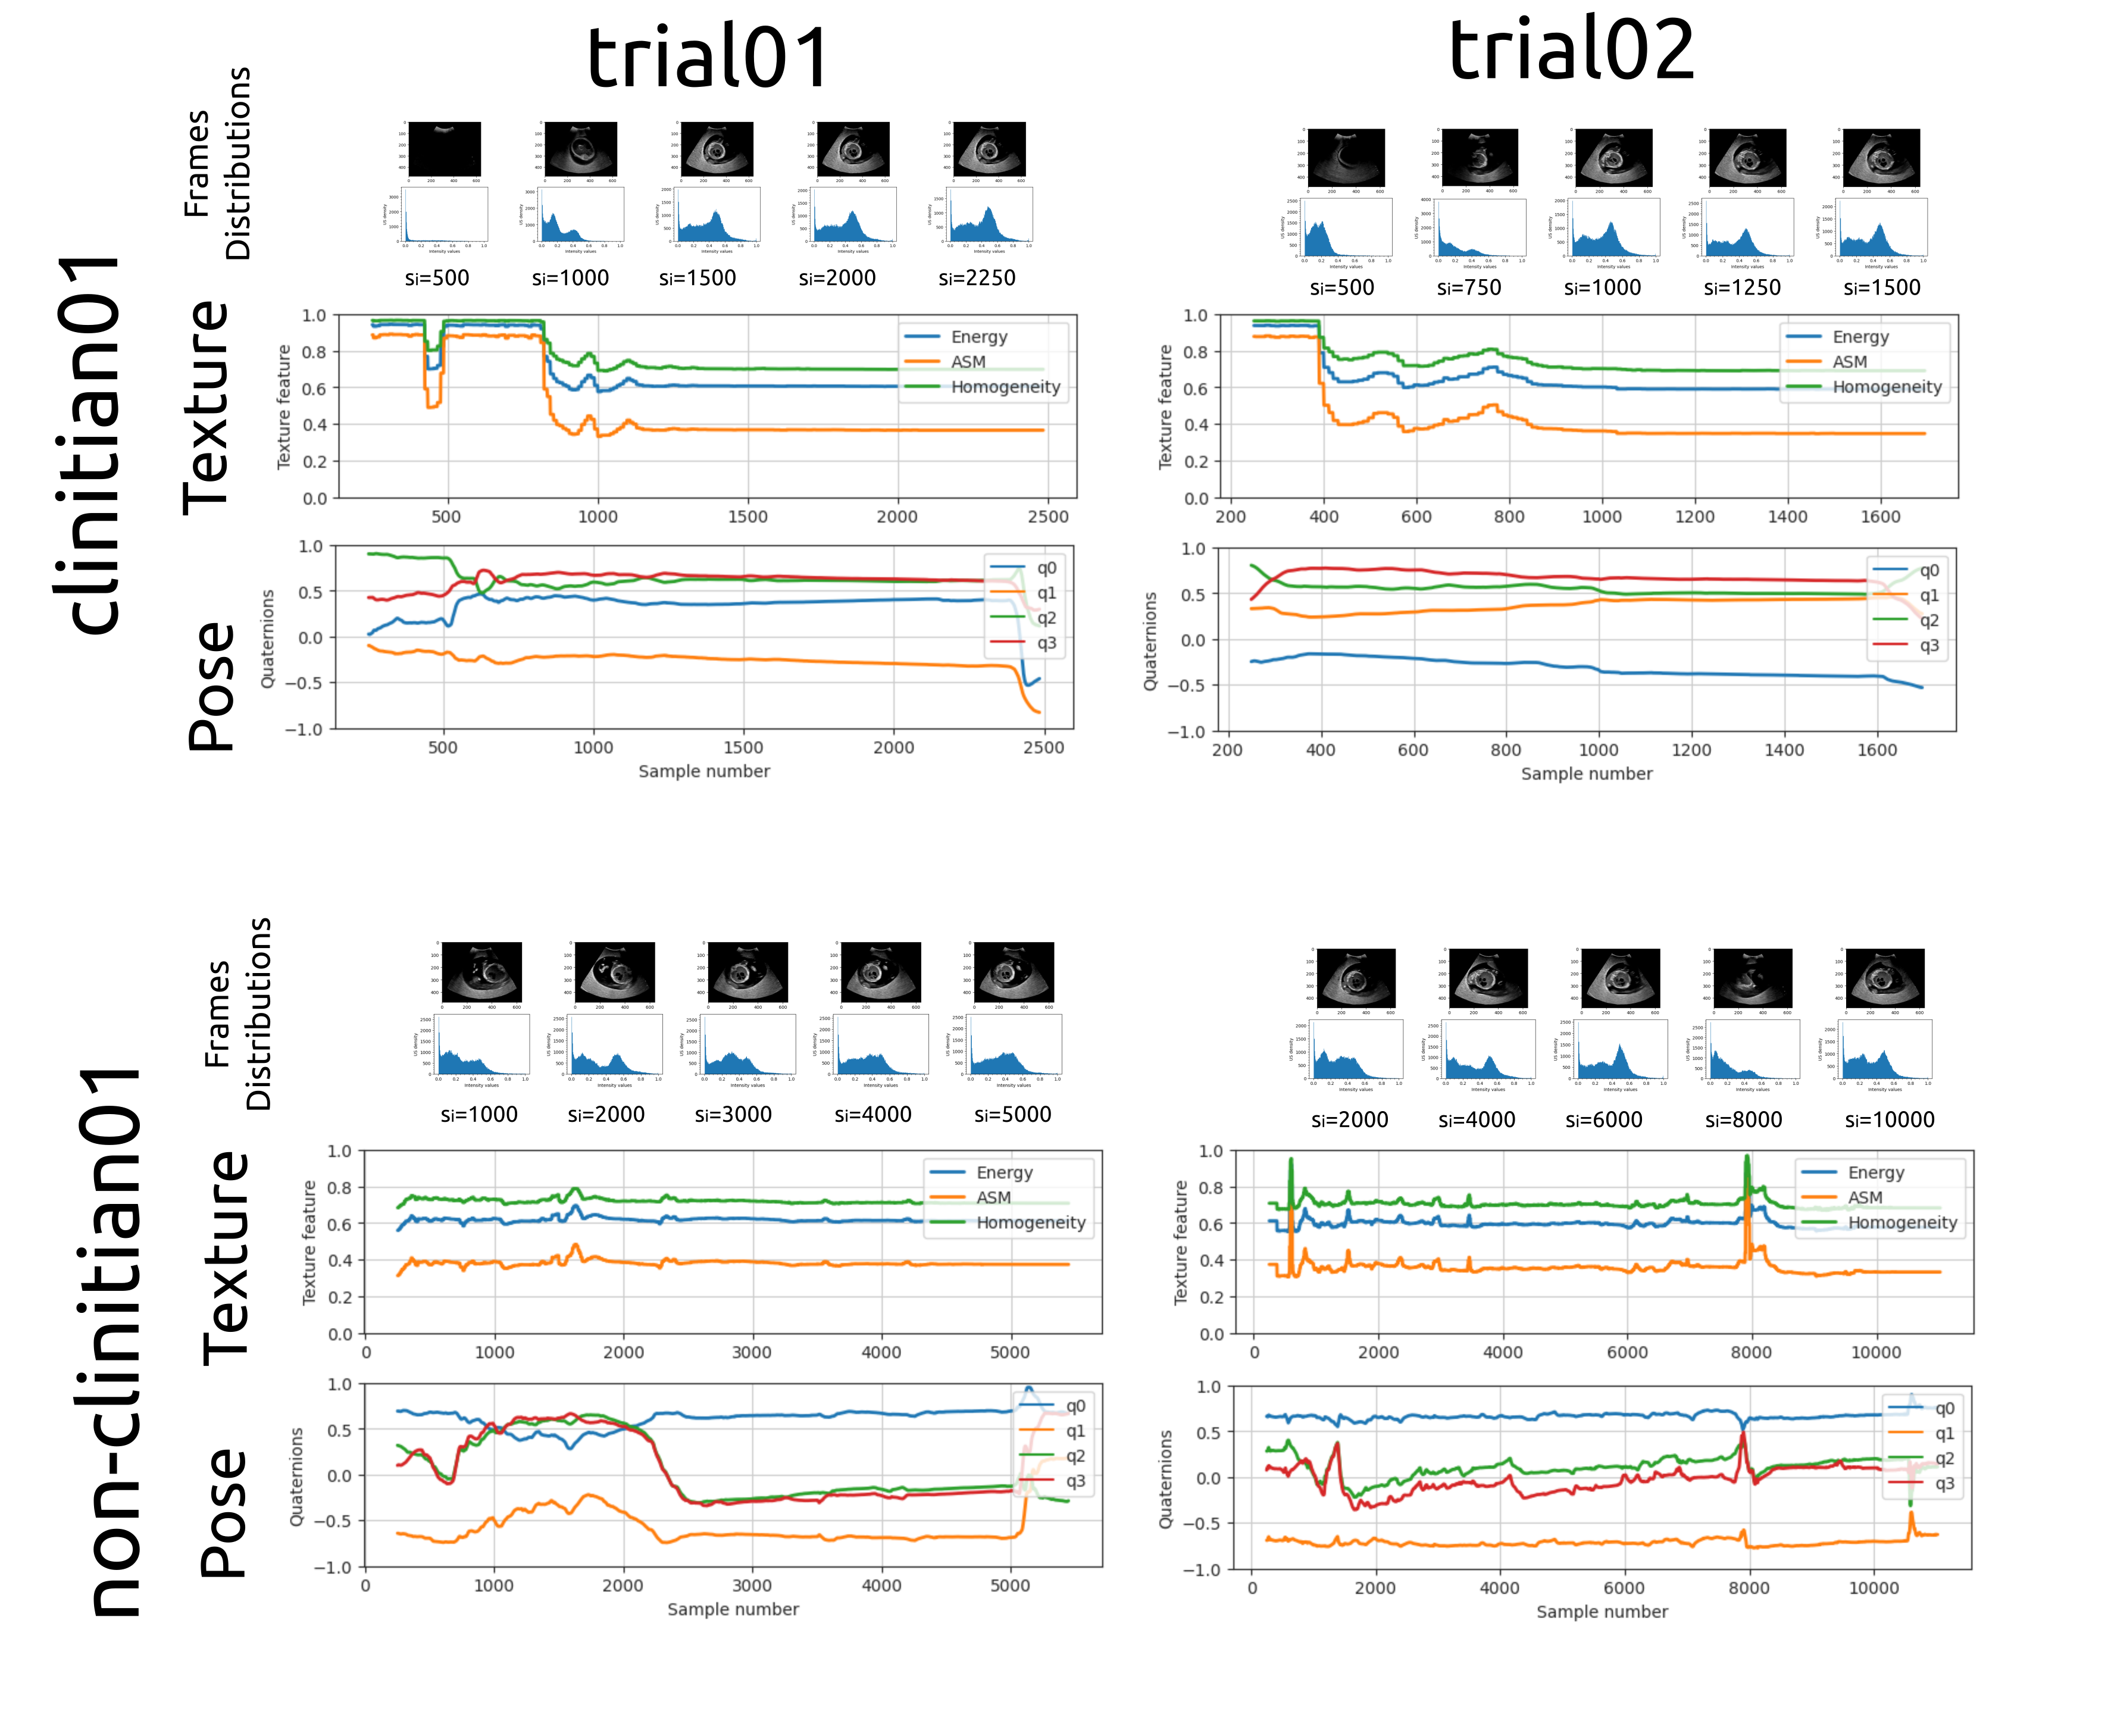
\includegraphics[width=0.44\textwidth]{fig-results-02-participants-02-trials.png} %%OVERLEAF and ARXIV
\caption{
Ultrasound image frames, image distributions, image texture features (energy, Angular Second Momentum ASM, and homogeneity) and pose time-series (quaternions) from one experienced clinician (clinician01) and one non-clinician (non-clinician01) in two trials (trial01 and trial02), looking for four-chamber optimal scanning plane. 
       } 
\label{fig:results}
% \end{figure*}
\end{figure}
%%---------------------------------(FIGURE)------------------------------------

%\subsection{Figures and Tables}
%Positioning Figures and Tables: Place figures and tables at the top and bottom of columns. Avoid placing them in the middle of columns. 
%Large figures and tables may span across both columns. 
%Figure captions should be below the figures; table heads should appear above the tables. 
%Insert figures and tables after they are cited in the text. 
%Use the abbreviation Fig. 1, even at the beginning of a sentence.
%\begin{table}[h]
%\caption{An Example of a Table}
%\label{table_example}
%\begin{center}
%\begin{tabular}{|c||c|}
%\hline
%One & Two\\
%\hline
%Three & Four\\
%\hline
%\end{tabular}
%\end{center}
%\end{table}
 
\section{CONCLUSIONS AND FUTURE WORK}
We have presented a simple framework of skill transfer learning for robotic ultrasound-guidance procedures.
We presented sensor fusion methods and sampling rate techniques for optimal scanning plane of the four-chamber view from two participants (one experienced clinician and one non-clinicians), where experienced clinician showed an smother and quicker procedure compare to a lengthy and non-constant movement of non-clinician.
For future work, we pointed out the need of pruned and quantised neural network models for real-time applications in robotic ultrasound-guidance procedure. 
% and a reproducible software/hardware pipeline to collect skills from clinicians to transfer them into a 
% simulated and r 

%%BLURS:FUTURE WORK 
%Hence, having appropriate methods to quantify such image and orientation quality in real-time leads with reliable clinical procedures is still an open challenge.
%NVIDIA Isaac Sim
%https://github.com/ArthurAllshire/HandTailor
%https://developer.nvidia.com/isaac-sim
%https://github.com/ankurhanda/dexpilot/tree/master

\addtolength{\textheight}{-12cm}   % This command serves to balance the column lengths
% on the last page of the document manually. It shortens
% the textheight of the last page by a suitable amount.
% This command does not take effect until the next page
% so it should come on the page before the last. Make
% sure that you do not shorten the textheight too much.

%%%%%%%%%%%%%%%%%%%%%%%%%%%%%%%%%%%%%%%%%%%%%%%%%%%%%%%%%%%%%%%%%%%%%%%%%%%%%%%%%
%\section*{APPENDIX}
%Appendixes should appear before the acknowledgment.

\section*{ACKNOWLEDGMENT}
Thanks to Tsz Yan Leung for her excellent research work  during her M.Sc. in Medical Physics and Engineering in 2022 at King's College London.
Thanks to Nhat Phung for volunteering as experienced sonographer in the experiments to identify optimal scanning plane of fetal four-chamber views at St Thomas' Hospital. 

%%%%%%%%%%%%%%%%%%%%%%%%%%%%%%%%%%%%%%%%%%%%%%%%%%%%%%%%%%%%%%%%%%%%%%%%%%%%%%%%
\bibliographystyle{IEEEtran}
% \bibliography{../references/references}%%LOCAL/GITHUB
%\bibliography{references}%%OVERLEAF
% \bibliography{../../references/references}%%ARXIV
%%%
%%%
%%%
%%%%%%%%%%%%%%%%%%%%%%%%%%%%%%%%%%%%%%%%%%%%%%%%%%%%%
%%% Abstract for Robotic-Assisted Medical Imaging 
%%% [LINK]: https://sites.google.com/view/rami-icra-2023-workshop/home
%%% Important dates 
%%% Abstract Submission Deadline: ~15th March 2023~, 24th March 2023
%%% Author Notification: 1st April 2023
%%% Workshop Date: 29th May 2023
%%%
%%%
%%% 
%%%%%%%%%%%%%%%%%%%%%%%%%%%%%%%%%%%%%%%%%%%%%%%%%%%%%
%%% Instructions for overleaf project
%%% Overleaf might be new to you, but it is quite easy to use. 
%%% 1. Go to the section where you want to write up or to edit in the PDF paper and double click that will point you to the text editor. 
%%% 2. Make edition as in word, and
%%% 3. Press Ctrl+s to save and compile your changes in the PDF document.
%%% 4. After Ctrl+s, all should be saved and ready for others to see, to review, etc.
%%% Ps. Using percentage symbol is considered as comment and it is not appearing in the PDF version of the paper.
%%% Don't worry about adding new references `\cite{}`, we can add them later.
%%% Thanks, Miguel
%%%
%%%
%%%%%%%%%%%%%%%%%%%%%%%%%%%%%%%%%%%%%%%%%%%%%%%%%%%%%
%%% Github repository:
%%% The resources to reproduce this work are available at 
%%% [LINK]: https://github.com/mxochicale/rami-icra2023
%%%
%%%
%%%


%%%%%%%%%%%%%%%%%%%%%%%%%%%%%%%%%%%%%%%%%%%%%%%%%%%%%%%%%%%%%%%%%%%%%%%%%%%%%%%%
%2345678901234567890123456789012345678901234567890123456789012345678901234567890
%        1         2         3         4         5         6         7         8

%\documentclass[letterpaper, 10 pt, conference]{ieeeconf}  % Comment this line out if you need a4paper

\documentclass[a4paper, 10pt, conference]{ieeeconf}      % Use this line for a4 paper

\IEEEoverridecommandlockouts             % This command is only needed if 
% you want to use the \thanks command

\overrideIEEEmargins                                      % Needed to meet printer requirements.

%In case you encounter the following error:
%Error 1010 The PDF file may be corrupt (unable to open PDF file) OR
%Error 1000 An error occurred while parsing a contents stream. Unable to analyze the PDF file.
%This is a known problem with pdfLaTeX conversion filter. The file cannot be opened with acrobat reader
%Please use one of the alternatives below to circumvent this error by uncommenting one or the other
%\pdfobjcompresslevel=0
%\pdfminorversion=4

% See the \addtolength command later in the file to balance the column lengths
% on the last page of the document

% The following packages can be found on http:\\www.ctan.org
%\usepackage{graphics} % for pdf, bitmapped graphics files
%\usepackage{epsfig} % for postscript graphics files
%\usepackage{mathptmx} % assumes new font selection scheme installed
%\usepackage{times} % assumes new font selection scheme installed
%\usepackage{amsmath} % assumes amsmath package installed
%\usepackage{amssymb}  % assumes amsmath package installed
\usepackage{graphicx}
\graphicspath{{../figures}} 
%\usepackage[hidelinks]{hyperref}
\usepackage{hyperref}
\hypersetup{
    colorlinks=false,
    pdfborder={0 0 0}
}

\title{\LARGE \bf
%Towards automatic ultrasound-guidance procedures. %Added: Thu 23 Feb 16:08:53 GMT 2023
%Learning ultrasound-guidance procedures. %Added: Thu 23 Feb 16:08:53 GMT 2023
%Towards AI-based ultrasound-guidance procedures %Mon 27 Feb 17:55:33 GMT 2023
%Learning and quantifying ultrasound-guidance procedures %Mon 27 Feb 17:57:32 GMT 2023
%Towards the Skill Transfer Learning of Ultrasound-guidance Procedures %Mon  6 Mar 00:23:54 GMT 2023
%Learning Skills of Ultrasound-guidance procedures  %Mon  6 Mar 00:41:51 GMT 2023
%Towards Skill Transfer Learning of Ultrasound-guidance Procedures %Mon  6 Mar 18:39:17 GMT 2023
%%
%Towards Reproducible Skill Transfer Learning 
%%Hardware and Software 
%Framework of Ultrasound-guidance Procedures %Mon  6 Mar 19:10:51 GMT 2023
%%
%Towards Reproducible Frameworks for Skill Transfer Learning of Ultrasound-guidance Procedures %Wed 15 Mar 17:41:03 GMT 2023
%Towards Reproducible Frameworks for Skill Transfer Learning of Robotic Ultrasound-guidance Procedures %Fri 17 Mar 17:15:29 GMT 2023
%Towards Simpler Frameworks for Skill Transfer Learning of \\ Robotic Ultrasound-guidance Procedures %Sat 18 Mar 23:43:33 GMT 2023
% Towards Simpler Frameworks of Skill Transfer Learning for \\ Robotic Ultrasound-guidance Procedures %Sun 19 Mar 00:14:16 GMT 2023
% Towards a Framework of Skill Transfer Learning for \\ Robotic Ultrasound-guidance Procedures %Sat 25 Mar 09:00:24 GMT 2023
Towards a Simple Framework of Skill Transfer Learning for \\ Robotic Ultrasound-guidance Procedures %Tue 28 Mar 23:11:49 BST 2023
}

\author{Tsz Yan Leung$^{1}$ and Miguel Xochicale$^{2}$% <-this % stops a space
% \author{[ADD CO-AUTHORS] and Miguel Xochicale$^{2}$% <-this % stops a space
%\thanks{*This work was not supported by any organization}% <-this % stops a space
\thanks{$^{1}$
	King's College London, UK
       {\tt\small tsz\_yan.leung@kcl.ac.uk}}%
\thanks{$^{2}$
	Currently University College London, UK. 
        Previously King's College London, UK.
        {\tt\small m.xochicale@ucl.ac.uk}}%
}


\begin{document}
\maketitle
\thispagestyle{empty}
\pagestyle{empty}


%%%%%%%%%%%%%%%%%%%%%%%%%%%%%%%%%%%%%%%%%%%%%%%%%%%%%%%%%%%%%%%%%%%%%%%%%%%%%%%%
\begin{abstract}
In this paper, we present a simple framework of skill transfer learning for robotic ultrasound-guidance procedures.
We briefly review challenges in skill transfer learning for robotic ultrasound-guidance procedures.
We then identify the need of appropriate sampling techniques, computationally efficient neural networks models that lead to the proposal of a simple framework of skill transfer learning for real-time applications in robotic ultrasound-guidance procedures.
We present pilot experiments from two participants (one experienced clinician and one non-clinician) looking for an optimal scanning plane of the four-chamber cardiac view from a fetal phantom.
We analysed ultrasound image frames, time series of texture image features and quaternions and found that the experienced clinician performed the procedure in a quicker and smoother way compared to lengthy and non-constant movements from non-clinicians.
For future work, we pointed out
the need of pruned and quantised neural network models
for real-time applications in robotic ultrasound-guidance
procedure.
The resources to reproduce this work are available at \url{https://github.com/mxochicale/rami-icra2023}.
\end{abstract}


%%%KEYWORDS 
% Image-guided intervention
% Robotic US imaging
% Autonomous medical imaging system

%%%%%%%%%%%%%%%%%%%%%%%%%%%%%%%%%%%%%%%%%%%%%%%%%%%%%%%%%%%%%%%%%%%%%%%%%%%%%%%%
\section{INTRODUCTION}
Ultrasound (US) imaging is a popular imaging modality because of its affordability, 
non-ionising imaging, and real-time capabilities.
Recently, the field of ultrasound-guidance procedures has been advanced with the development of robotic ultrasound systems that range from tele-operated, semi-autonomous and fully autonomous~\cite{deng2021, vonHaxthausen2021, Gerlach2022}. 
% Ipsen2021 leave out for future work
However, there are still scientific and technical challenges in robotic ultrasound-guidance procedures: 
(a) traditional imaging is user-dependent, skill-dependant and device-dependent \cite{chen1997},
(b) traditional hardware for human motion tracking is usually expensive or cumbersome~\cite{Dressler2021}, and 
(c) frameworks are designed for specific types of sensors, clinical US devices, robots and operating systems~\cite{niu2022}.
Learning ultrasound skills from sonographers that look for the optimal scanning plane (OSP) is still an open challenge in robotic ultrasound-guidance procedures~\cite{deng2021}.
It is hypothesised that robotic ultrasound-guided procedures would require to be simple, less expensive and less cumbersome for skill transfer learning.
Hence, in this paper, we are proposing a simple framework of skill transfer learning for robotic ultrasound-guidance procedures.
This paper is divided into robotic ultrasound-guidance procedures, framework for sonographer skill transfer learning, results and conclusions with future work.

% \section{SIMPLE FRAMEWORK OF SONOGRAPHER SKILL TRANSFER LEARNING FOR ROBOTIC ULTRASOUND-GUIDANCE PROCEDURES}
\section{ROBOTIC ULTRASOUND-GUIDANCE PROCEDURES}
Robotic ultrasound systems are actively investigated for teleoperatation, semi-autonomous and fully autonomous modalities~\cite{vonHaxthausen2021}.
For instance, Deng et al. proposed a multi-modal task learning architecture for ultrasound scanning skills with input data from ultrasound images, force and probe pose, stating the challenge of real-time guidance due to computational signal processing~\cite{deng2021}.
Robotic US-guidance radiation therapy for lesion in abdomen has been successful using CNN-based search.
However, treatment plans without US-robot guidance are still superior to robotic US-guidance because of the quality of acquired ultrasound images~\cite{Gerlach2022}.
% Recently, robotic minimally invasive surgery has been investigated with silica gel phantoms where the optical tracking system, from Vicon Motion Systems Ltd, was prone to deviations due to light occlusions~\cite{niu2022}.

%%---------------------------------(FIGURE)-------------------------------------
\begin{figure}[t]
\centering
% \includegraphics[width=0.47\textwidth]{framework/outputs/drawing-v00} %%LOCAL/GITHUB
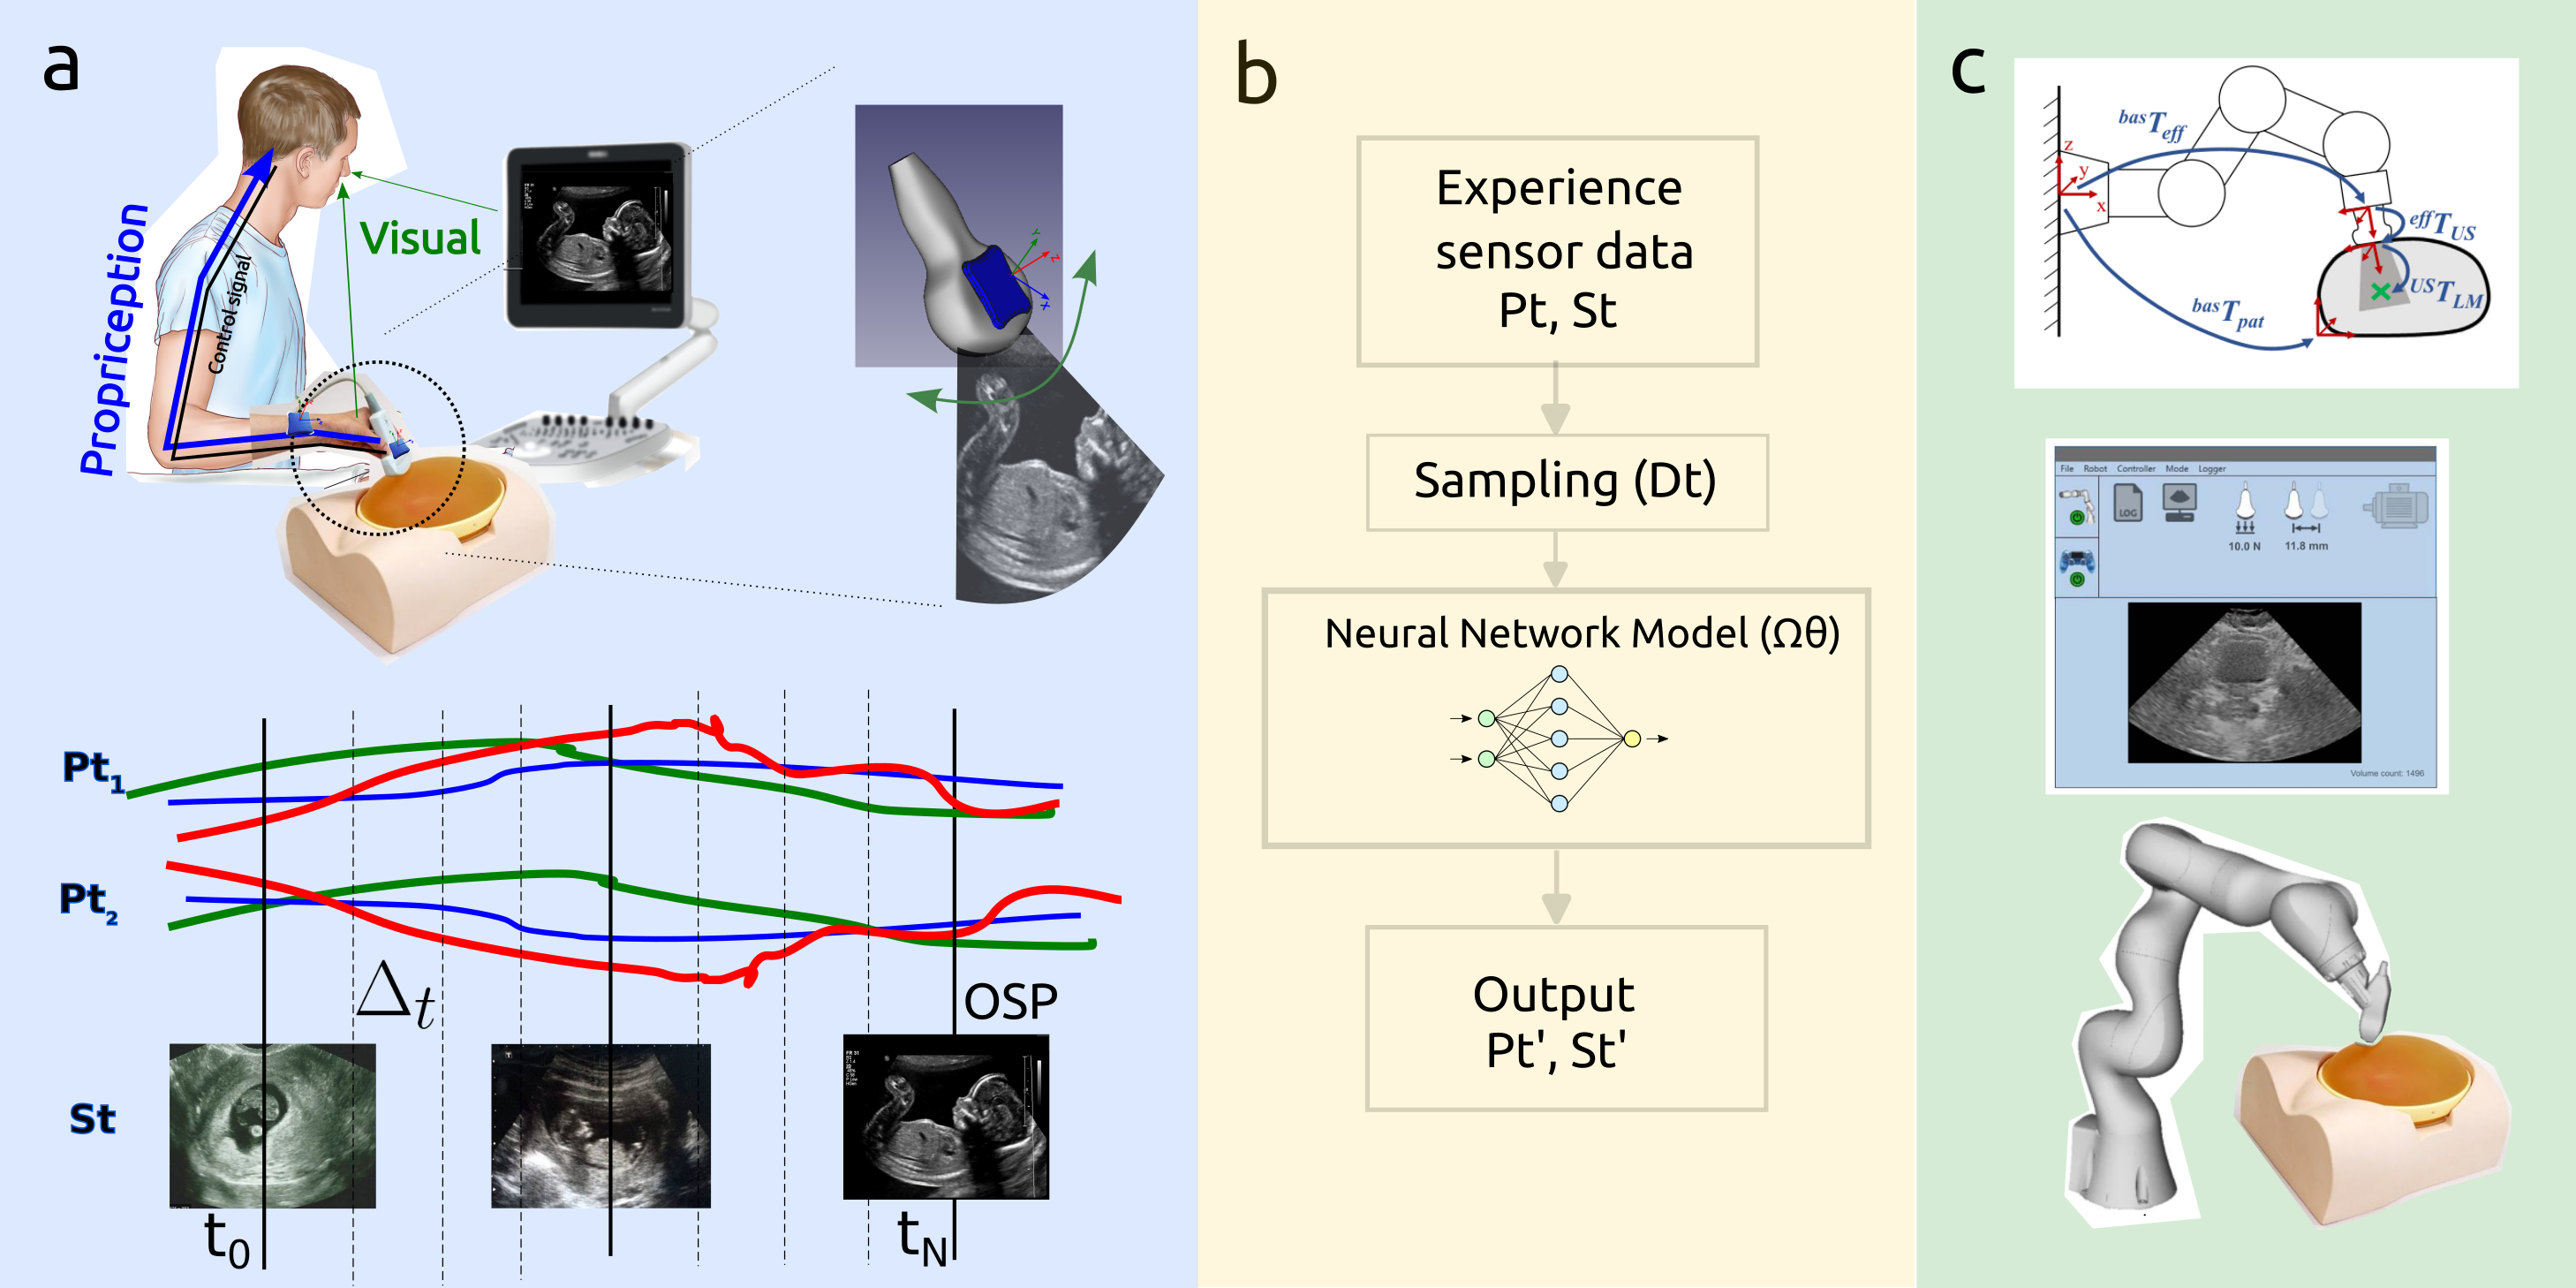
\includegraphics[width=0.47\textwidth]{fig-framework.png} %%OVERLEAF and ARXIV
    \caption{
            \textbf{(a)} Ultrasound-guidance procedures:
		sonographer operating an ultrasound machine with fetal phantom and sensor fusion signals from inertial sensors and ultrasound imaging;
            \textbf{(b)} Simple framework for skill transfer learning: 
		collecting experience with sensors ($Pt_n$ pose and $St$ Signal), sampling method for fusion sensor ($\Delta_t$), and identified the need of computational efficient neural network model ($\Omega_\theta$), and output for high-dimensional model ~\cite{deng2021}, and 
            %\textbf{(c)} 
            \textbf{(c)} Robotic ultrasound-guidance procedures:
		transformations, graphical user interface and simulation using robotic US-guidance light-weight 7 degrees-of-freedom robot (KUKA LBR Med 7)~\cite{Gerlach2022, Ipsen2021}.
       }
\label{fig:main}
\end{figure}
%%---------------------------------(FIGURE)------------------------------------

%%BLURS
%reproducible frameworks to address challenges on sustainability, reproducibly and good software/hardware practices.
%still be robustified by simplifying and making more effective procedures. 
%TOREVIEW~\cite{Ipsen2021}. 


\section{FRAMEWORK FOR SONOGRAPHER SKILL TRANSFER LEARNING}
%\subsection{Fusion-sensors}
Modelling the optimal scanning plane (OSP) requires ultrasound images, spacial locations and anatomical understanding from experienced sonographers (Fig~\ref{fig:main}a)~\cite{deng2021,vonHaxthausen2021}.
Current systems to model OPS are expensive and cumbersome leading to the need of smaller and low-cost systems~\cite{Dressler2021}. 
% This leads to systems that are expensive and 
% the need for simpler, affordable and less invasive framework for skill transfer learning. 
One potential avenue to reduce cost and ergonomic form factor is (a) the use of Inertial Measurement Units (IMU) to track probe position during US scanning procedures~\cite{PREVOST2018187}
and (b) the application of the appropriate fusion techniques of ultrasound video signal and motion signal from IMU for probe guidance~\cite{droste2020}, and (c) computationally efficient neural networks models~\cite{deng2021}.
Hence, we introduce a framework for sonographer skills transfer learning, considering: sampling technique and fusion sensor techniques (IMU and US) and discuss the need of real-time guidance with  pruned and quantised neural network models, feature extraction and transfer learning for robotic-ultrasound-guidance procedures (Fig~\ref{fig:main}b, c).
%%%BLURS

% Recently, Deng et al. investigated ultrasound skill learning with VGG-16 and fully connected layers by modelling relationships among US images, the probe pose and the contact force~\cite{deng2021}.
% However, real-time guidance is still a challenge due appropriate sampling techniques and the computational cost for large sensor samples.
% Hence, to address previous challenges in skill transfer learning, 

%Hence, considering the current trends towards the use of portable US scanners \cite{PREVOST2018187}.
%Droste et al. proposed a probe guidance system fusing 
%%was investigated to predict movement towards either the standard plane position or the next performed movements of a sonographer 

%%Similarly, having portable and non-obstrusive devices to track such image/orienation quality leads to essier clinical procedures [ADDREF].
%because of its small food print as well as the advantage oe being less expensive or add challenges in obstructions or magnetic disturbances.

%TOREVIEW 
%https://www.clinicalimaging.org/article/S0899-7071(21)00405-8/fulltext
%https://onlinelibrary.wiley.com/doi/abs/10.1002/jcu.23431?casa_token=Mq5YVW9UtLYAAAAA%3ARZ2sq111NUVdRyBDiTfWMdfWVtgoeTbAvw-DXPV5zwUD5IWzuu7VLAU2OgHEGobc0CO0b-S7Y2xQSaM
%https://aapm.onlinelibrary.wiley.com/doi/epdf/10.1002/mp.15432

\section{EXPERIMENTS: DESIGN AND RESULTS}
\subsection{Experiment setup}
Considering fetal biometry parameters from the NHS 20-week screening scan protocol and National Health Service (NHS) foetal anomaly screening programme (FASP)~\cite{NHS_england2022},
% NICE2022
we conducted a pilot experiment with two participants (one non-clinical and one clinical with 10 years of experience in echocardiography).
During the experiment, we asked participants to find the optimal scanning plane for the four chamber view of foetal ultrasound examination phantom ("SPACE FAN-ST", Kyoto Kagaku Co., Ltd, Kyoto, Japan).
We attached inertial sensors (LPMS-B2, LP-Research Inc., Tokyo, Japan) to a convex US probe to track the pose of the ultrasound image from a clinical ultrasound device (EPIQ 7G, Koninklijke Philips N.V., Amsterdam, Netherlands) with the use of a CPU laptop computer that streamed images via a USB framegrabber (Mirabox).

\subsection{Experimental results}
Fig~\ref{fig:results} shows the time series from one experienced clinician and one non-clinician while looking for an optimal scanning plane of the four-chamber view.
It can be noted that the expert took less time (1600 and 2500 samples) to find an optimal scanning plane whereas non-clinician took a greater time (5000 and 10000 samples).
Similarly, the time-series for the experienced clinician appear to be more smooth and consistent compared to the jerkiness of non-clinical participant. 
%%---------------------------------(FIGURE)-------------------------------------
\begin{figure}[t]
% \begin{figure*}[th] % two-column figure on desired page
\centering
% \includegraphics[width=0.44\textwidth]{results-02-participants-02-trials/outputs/drawing-v00} %%LOCAL/GITHUB
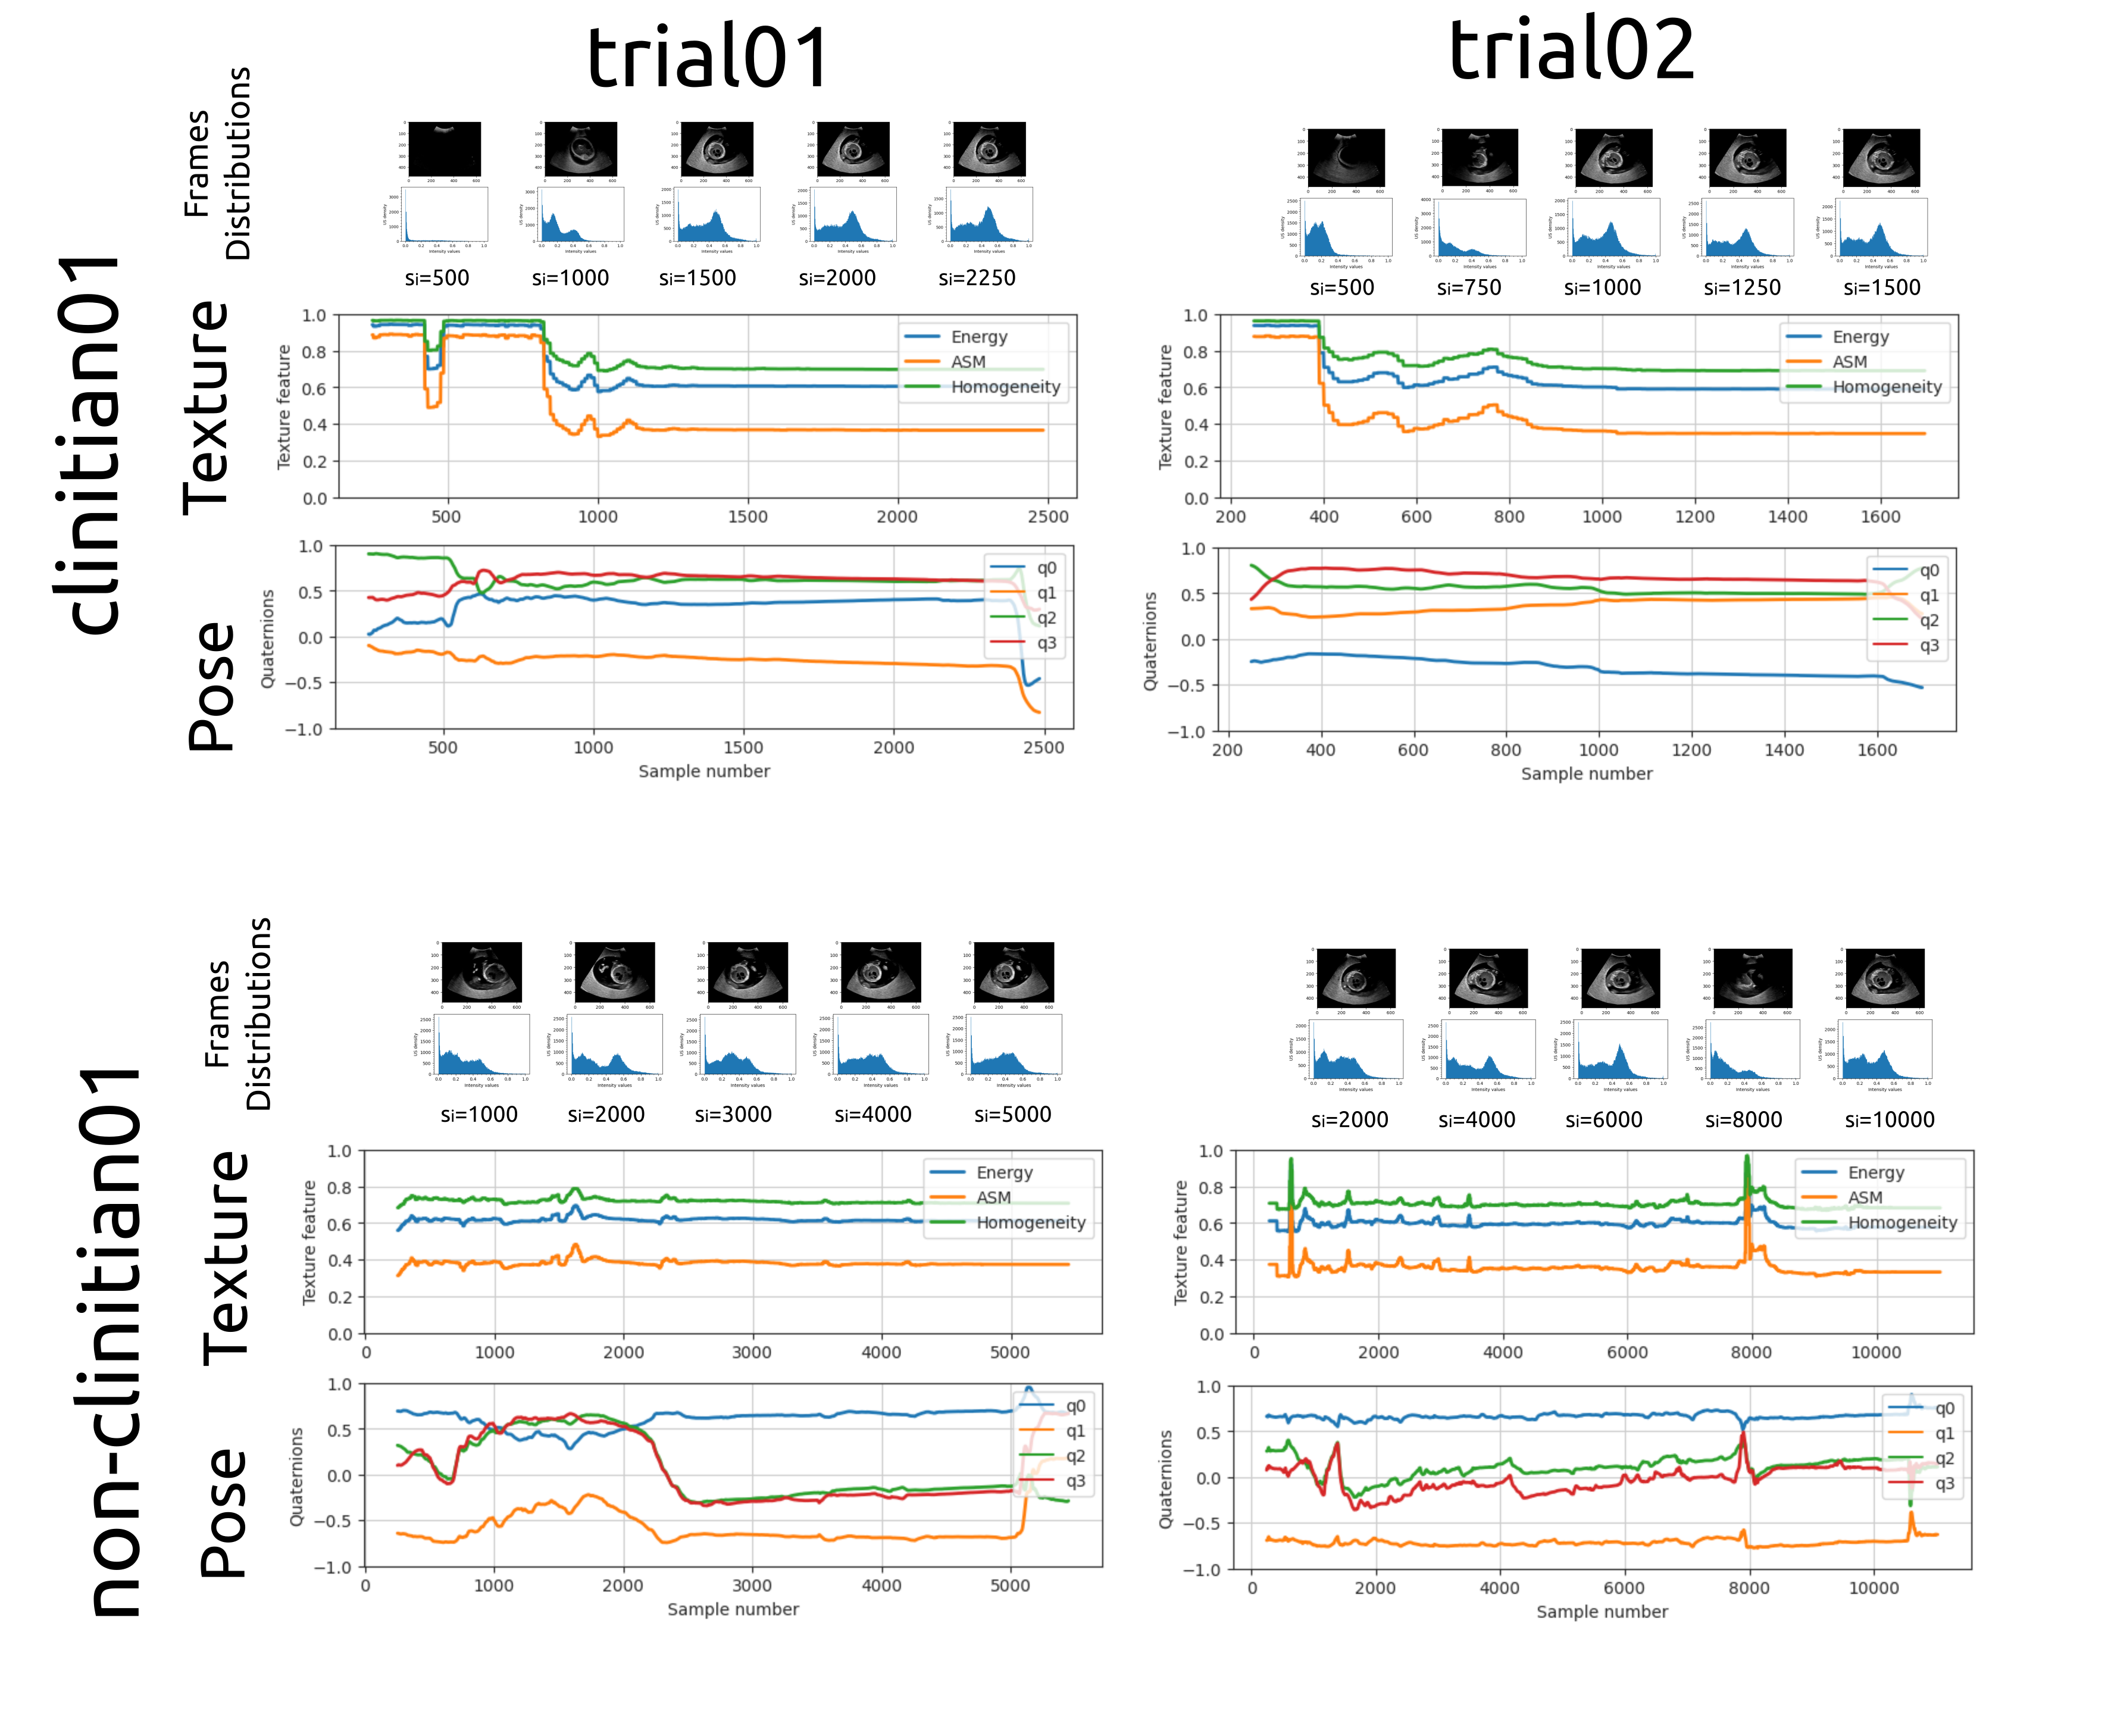
\includegraphics[width=0.44\textwidth]{fig-results-02-participants-02-trials.png} %%OVERLEAF and ARXIV
\caption{
Ultrasound image frames, image distributions, image texture features (energy, Angular Second Momentum ASM, and homogeneity) and pose time-series (quaternions) from one experienced clinician (clinician01) and one non-clinician (non-clinician01) in two trials (trial01 and trial02), looking for four-chamber optimal scanning plane. 
       } 
\label{fig:results}
% \end{figure*}
\end{figure}
%%---------------------------------(FIGURE)------------------------------------

%\subsection{Figures and Tables}
%Positioning Figures and Tables: Place figures and tables at the top and bottom of columns. Avoid placing them in the middle of columns. 
%Large figures and tables may span across both columns. 
%Figure captions should be below the figures; table heads should appear above the tables. 
%Insert figures and tables after they are cited in the text. 
%Use the abbreviation Fig. 1, even at the beginning of a sentence.
%\begin{table}[h]
%\caption{An Example of a Table}
%\label{table_example}
%\begin{center}
%\begin{tabular}{|c||c|}
%\hline
%One & Two\\
%\hline
%Three & Four\\
%\hline
%\end{tabular}
%\end{center}
%\end{table}
 
\section{CONCLUSIONS AND FUTURE WORK}
We have presented a simple framework of skill transfer learning for robotic ultrasound-guidance procedures.
We presented sensor fusion methods and sampling rate techniques for optimal scanning plane of the four-chamber view from two participants (one experienced clinician and one non-clinicians), where experienced clinician showed an smother and quicker procedure compare to a lengthy and non-constant movement of non-clinician.
For future work, we pointed out the need of pruned and quantised neural network models for real-time applications in robotic ultrasound-guidance procedure. 
% and a reproducible software/hardware pipeline to collect skills from clinicians to transfer them into a 
% simulated and r 

%%BLURS:FUTURE WORK 
%Hence, having appropriate methods to quantify such image and orientation quality in real-time leads with reliable clinical procedures is still an open challenge.
%NVIDIA Isaac Sim
%https://github.com/ArthurAllshire/HandTailor
%https://developer.nvidia.com/isaac-sim
%https://github.com/ankurhanda/dexpilot/tree/master

\addtolength{\textheight}{-12cm}   % This command serves to balance the column lengths
% on the last page of the document manually. It shortens
% the textheight of the last page by a suitable amount.
% This command does not take effect until the next page
% so it should come on the page before the last. Make
% sure that you do not shorten the textheight too much.

%%%%%%%%%%%%%%%%%%%%%%%%%%%%%%%%%%%%%%%%%%%%%%%%%%%%%%%%%%%%%%%%%%%%%%%%%%%%%%%%%
%\section*{APPENDIX}
%Appendixes should appear before the acknowledgment.

\section*{ACKNOWLEDGMENT}
Thanks to Tsz Yan Leung for her excellent research work  during her M.Sc. in Medical Physics and Engineering in 2022 at King's College London.
Thanks to Nhat Phung for volunteering as experienced sonographer in the experiments to identify optimal scanning plane of fetal four-chamber views at St Thomas' Hospital. 

%%%%%%%%%%%%%%%%%%%%%%%%%%%%%%%%%%%%%%%%%%%%%%%%%%%%%%%%%%%%%%%%%%%%%%%%%%%%%%%%
\bibliographystyle{IEEEtran}
% \bibliography{../references/references}%%LOCAL/GITHUB
%\bibliography{references}%%OVERLEAF
% \bibliography{../../references/references}%%ARXIV
\input{main.bbl} %% uncomment for arxiv version

\end{document}
 %% uncomment for arxiv version

\end{document}
 %% uncomment for arxiv version

\end{document}
 %% uncomment for arxiv version

\end{document}
